%%%%%%%%%%%%%%%%%%%%%%%%%%%%%%%%%%%%%%%%%%%%%%%%%%%%%%%%%%%%%%%%%%%%%%%%%%%%%%%%
%% Plantilla de memoria en LaTeX para la ETSIT - Universidad Rey Juan Carlos
%%
%% Por Gregorio Robles <grex arroba gsyc.urjc.es>
%%     Grupo de Sistemas y Comunicaciones
%%     Escuela Técnica Superior de Ingenieros de Telecomunicación
%%     Universidad Rey Juan Carlos
%% (muchas ideas tomadas de Internet, colegas del GSyC, antiguos alumnos...
%%  etc. Muchas gracias a todos)
%%
%% La última versión de esta plantilla está siempre disponible en:
%%     https://github.com/gregoriorobles/plantilla-memoria
%%
%% Para obtener PDF, ejecuta en la shell:
%%   make
%% (las imágenes deben ir en PNG o JPG)

%%%%%%%%%%%%%%%%%%%%%%%%%%%%%%%%%%%%%%%%%%%%%%%%%%%%%%%%%%%%%%%%%%%%%%%%%%%%%%%%

\documentclass[a4paper, 12pt]{book}
%\usepackage[T1]{fontenc}

\usepackage[a4paper, left=2.5cm, right=2.5cm, top=3cm, bottom=3cm]{geometry}
\usepackage{times}
\usepackage[latin1]{inputenc}
\usepackage[spanish]{babel} % Comenta esta línea si tu memoria es en inglés
\usepackage{url}
%\usepackage[dvipdfm]{graphicx}
\usepackage{graphicx}
\usepackage{float}  %% H para posicionar figuras
\usepackage[nottoc, notlot, notlof, notindex]{tocbibind} %% Opciones de índice
\usepackage{latexsym}  %% Logo LaTeX
\usepackage{listings}

\title{Memoria del Proyecto}
\author{Nombre del autor}

\renewcommand{\baselinestretch}{1.5}  %% Interlineado

\begin{document}

\renewcommand{\refname}{Bibliografía}  %% Renombrando
\renewcommand{\appendixname}{Apéndice}

%%%%%%%%%%%%%%%%%%%%%%%%%%%%%%%%%%%%%%%%%%%%%%%%%%%%%%%%%%%%%%%%%%%%%%%%%%%%%%%%
% PORTADA

\begin{titlepage}
\begin{center}
\begin{tabular}[c]{c c}
%\includegraphics[bb=0 0 194 352, scale=0.25]{logo} &
\includegraphics[scale=0.25]{img/logo_vect.png} &
\begin{tabular}[b]{l}
\Huge
\textsf{UNIVERSIDAD} \\
\Huge
\textsf{REY JUAN CARLOS} \\
\end{tabular}
\\
\end{tabular}

\vspace{3cm}

\Large
GRADO EN INGENIERÍA DE SISTEMAS AUDIOVISUALES Y MULTIMEDIA

\vspace{0.4cm}

\large
Curso Académico 2016/2017

\vspace{0.8cm}

Trabajo Fin de Grado

\vspace{2.5cm}

\LARGE
HERRAMIENTA PARA EVALUAR LA CORRESPONDENCIA ENTRE MODELOS UML Y CÓDIGO FUENTE EN PROYECTOS PYTHON

\vspace{4cm}

\large
Autor : Cristian Álvarez Pérez \\
Tutor : Dr. Gregorio Robles
\end{center}
\end{titlepage}

\newpage
\mbox{}
\thispagestyle{empty} % para que no se numere esta pagina


%%%%%%%%%%%%%%%%%%%%%%%%%%%%%%%%%%%%%%%%%%%%%%%%%%%%%%%%%%%%%%%%%%%%%%%%%%%%%%%%
%%%% Para firmar
\clearpage
\pagenumbering{gobble}
\chapter*{}

\vspace{-4cm}
\begin{center}
\LARGE
\textbf{Trabajo Fin de Grado}

\vspace{1cm}
\large
Herramienta para Evaluar la Correspondencia Entre Modelos UML y Código Fuente en Proyectos Python

\vspace{1cm}
\large
\textbf{Autor :} Cristian Álvarez Pérez \\
\textbf{Tutor :} Dr. Gregorio Robles Martínez

\end{center}

\vspace{1cm}
La defensa del presente Proyecto Fin de Carrera se realizó el día \qquad$\;\,$ de marzo de 2017, siendo calificada por el siguiente tribunal:


\vspace{0.5cm}
\textbf{Presidente:}

\vspace{1.2cm}
\textbf{Secretario:}

\vspace{1.2cm}
\textbf{Vocal:}


\vspace{1.2cm}
y habiendo obtenido la siguiente calificación:

\vspace{1cm}
\textbf{Calificación:}


\vspace{1cm}
\begin{flushright}
Fuenlabrada, a \qquad$\;\,$ de marzo de 2017
\end{flushright}

%%%%%%%%%%%%%%%%%%%%%%%%%%%%%%%%%%%%%%%%%%%%%%%%%%%%%%%%%%%%%%%%%%%%%%%%%%%%%%%%
%%%% Dedicatoria

\chapter*{}
\pagenumbering{Roman} % para comenzar la numeracion de paginas en numeros romanos
\begin{flushright}
\textit{Dedicado a \\
mi familia y amigos, \\
que aunque no entienden nada de mi trabajo, \\
me entienden a mí.}
\end{flushright}

%%%%%%%%%%%%%%%%%%%%%%%%%%%%%%%%%%%%%%%%%%%%%%%%%%%%%%%%%%%%%%%%%%%%%%%%%%%%%%%%
%%%% Agradecimientos

\chapter*{Agradecimientos}
%\addcontentsline{toc}{chapter}{Agradecimientos} % si queremos que aparezca en el índice
\markboth{AGRADECIMIENTOS}{AGRADECIMIENTOS} % encabezado

Con la entrega de este trabajo pongo fin a una etapa, a unos años que han tenido momentos muy dispares, en lo que cada uno de ellos ha tenido algo bueno, aunque lo bueno fuera aprender de lo malo.

De estos años de carrera, quiero agradecer a mi familia por su comprensión a las horas que tenía que echar delante de un libro u ordenador, haciendo el mínimo ruido posible para no molestarme, y por sus pequeñas visitas para desconectar.
Quiero agradecer a mis amigos de toda la vida, por sus mensajes de apoyo el primer día de universidad y por sus mensajes de felicitación en el último.
También quiero agradecer a todas las personas que he conocido a lo largo de la carrera, desde la persona con la que me perdí en busca de nuestro primer aula el día de la presentación hasta con la que hable de que era nuestro último día de clase, sin olvidar a todos los demás que han estado entre medias, compartiendo horas de prácticas, trabajos, biblioteca, Skype... Todos por el mismo objetivo.

Respecto a mi TFG, quiero agradecer a todos los que me han ayudado directamente: con recomendaciones de cambios de palabra (tanto en inglés como en español), dándome una opinión general o simplemente, haciéndome compañía.
Y como no, a mi tutor Gregorio, por haberme dado la oportunidad de realizar este TFG y por haber estado tan atento contestando correos electrónicos a horas inesperadas.

Muchas gracias a todos, que aunque no os nombre, todos sabéis por quien va cada línea. Gracias.

%%%%%%%%%%%%%%%%%%%%%%%%%%%%%%%%%%%%%%%%%%%%%%%%%%%%%%%%%%%%%%%%%%%%%%%%%%%%%%%%
%%%% Resumen

\chapter*{Resumen}
%\addcontentsline{toc}{chapter}{Resumen} % si queremos que aparezca en el índice
\markboth{RESUMEN}{RESUMEN} % encabezado

El presente trabajo tiene como objetivo la creación de una aplicación web para ofrecer métricas respecto a la correspondencia de código Python con diagramas en UML. De esta manera, se
podrá obtener un valor de representación de UML en Python. Los resultados obtenidos
podrían servir para conocer cuál es el uso que se le da a UML en un proyecto.

La aplicación web se ha desarrollado con tecnologías HTML5, BootStrap y CSS3
en el lado del cliente, y con tecnologías Django, Ctags y Python en el lado del servidor.
En la actualidad está orientada al análisis de proyectos en GitHub, pero su uso se puede generalizar a cualquier otra plataforma.

La correspondencia en cuanto a representación de código y diagramas UML permite conocer mejor el uso que los desarrolladores hacen del modelado, pudiendo identificarse errores, patrones de conducta, inconsistencias, etc. Para mostrar la conveniencia de la aplicación que se ha creado en este TFG, se ha aplicado a 108 proyectos Python alojados en GitHub que contienen diagramas UML.


%%%%%%%%%%%%%%%%%%%%%%%%%%%%%%%%%%%%%%%%%%%%%%%%%%%%%%%%%%%%%%%%%%%%%%%%%%%%%%%%
%%%% Resumen en inglés

\chapter*{Summary}
%\addcontentsline{toc}{chapter}{Summary} % si queremos que aparezca en el índice
\markboth{SUMMARY}{SUMMARY} % encabezado

This graduate thesis aims to create a web application to provide metrics regarding the correspondence of Python code with diagrams in UML. In this way, it is possible to obtain a UML representation value for Python projects. The results obtained could serve to know what is the use that is given to UML in a project.

The web application has been developed with HTML5, BootStrap and CSS3 technologies on the client side, and with Django, Ctags and Python technologies on the server side. At present it is oriented to the analysis of projects in GitHub, but its use can be generalized to any other platform.

Correspondence in terms of code representation and UML diagrams allows us to better understand the use that developers make of modeling, being able to identify errors, behavior patterns, inconsistencies, etc. To show the convenience of the application that has been created in this TFG, it has been applied to 108 Python projects hosted in GitHub that contain UML diagrams.


%%%%%%%%%%%%%%%%%%%%%%%%%%%%%%%%%%%%%%%%%%%%%%%%%%%%%%%%%%%%%%%%%%%%%%%%%%%%%%%%
%%%%%%%%%%%%%%%%%%%%%%%%%%%%%%%%%%%%%%%%%%%%%%%%%%%%%%%%%%%%%%%%%%%%%%%%%%%%%%%%
% ÍNDICES %
%%%%%%%%%%%%%%%%%%%%%%%%%%%%%%%%%%%%%%%%%%%%%%%%%%%%%%%%%%%%%%%%%%%%%%%%%%%%%%%%

% Las buenas noticias es que los índices se generan automáticamente.
% Lo único que tienes que hacer es elegir cuáles quieren que se generen,
% y comentar/descomentar esa instrucción de LaTeX.

%%%% Índice de contenidos
\tableofcontents
%%%% Índice de figuras
\cleardoublepage
%\addcontentsline{toc}{chapter}{Lista de figuras} % para que aparezca en el indice de contenidos
\listoffigures % indice de figuras
%%%% Índice de tablas
%\cleardoublepage
%\addcontentsline{toc}{chapter}{Lista de tablas} % para que aparezca en el indice de contenidos
%\listoftables % indice de tablas



%%%%%%%%%%%%%%%%%%%%%%%%%%%%%%%%%%%%%%%%%%%%%%%%%%%%%%%%%%%%%%%%%%%%%%%%%%%%%%%%
%%%%%%%%%%%%%%%%%%%%%%%%%%%%%%%%%%%%%%%%%%%%%%%%%%%%%%%%%%%%%%%%%%%%%%%%%%%%%%%%
% INTRODUCCIÓN %
%%%%%%%%%%%%%%%%%%%%%%%%%%%%%%%%%%%%%%%%%%%%%%%%%%%%%%%%%%%%%%%%%%%%%%%%%%%%%%%%

\cleardoublepage
\chapter{Introducción}
\label{sec:intro} % etiqueta para poder referenciar luego en el texto con ~\ref{sec:intro}
\pagenumbering{arabic} % para empezar la numeración de página con números

\section{Motivación}
\label{sec:motivacion}

UML es un lenguaje de modelado que se enseña en multitud de universidades del mundo. Y, sin embargo, pese a ser ampliamente conocido, y a que es ampliamente aceptado en la industria del software, se ha observado que menos del 1\% de todos los repositorios almacenados en GitHub tienen su correspondiente representación en diagramas UML~\cite{hebig2016quest}.

Surge así el debate de por qué UML no es aceptado en entornos donde sería de gran ayuda. Uno de los problemas a los que se enfrenta UML es que, aún siendo de amplia difusión, es difícil encontrar ejemplos de proyectos reales donde se pueda ver su uso. Por tanto, en las universidades se enseña UML de manera muy teórica, limitándose la parte práctica a casos muy pequeños, podríamos decir \emph{de laboratorio}, muchas veces ajenos a la realidad de un proyecto software.

Para solucionar este problema, sería deseable contar con proyectos reales donde tuviéramos además su correspondiente diagrama UML. Esto serviría, además, para comprobar cómo se está modelando en proyectos reales, ya que en muchas ocasiones los diagramas que se utilizan en un entorno de desarrollo no contienen todos los detalles de implementación, sino que son una abstracción.

Por ello, surge la idea de este trabajo: una herramienta a la que se le indica la dirección URL de un proyecto en GitHub, y realice un análisis para poder evaluar la correspondencia en cuanto a código Python y su representación en diagramas de UML. Se decide utilizar Python para poder centrarse en un lenguaje concreto a modo concepto pero se puede extender a más lenguajes.

Se pretende dar apoyo al estudio realizado por la URJC, la Universidad de Gotemburgo y Chalmers University (Suecia) sobre el uso de UML, que tiene como objetivo analizar y fomentar el uso de UML en entornos de software libre. La asunción que hay detrás de estos esfuerzos es que el modelado permite crear mejores proyectos de software, ya que mejora la arquitectura del software, la comunicación entre el equipo de desarrollo y la documentación del proyecto. Por lo tanto, los resultados obtenidos con nuestra herramienta podrían ser asociados a la calidad del proyecto software, es decir, un proyecto que obtenga un porcentaje alto de representación en diagramas de UML tiene muchas posibilidades de ser a su vez un proyecto de calidad.

\section{Contexto}
\label{sec:contexto}

Actualmente, se han realizado varios estudios por las Universidades de Leiden (Países Bajos) y Universidad de Gotemburgo - Chalmers University, esta última en colaboración con la URJC, sobre el uso que se le da a UML en cuanto a sus representaciones. Estas investigaciones van dirigidas al estudio de modelización en proyectos de software libre~\cite{hebig2016quest}, la relación entre anti-patrones de diseño en diagramas UML y código fuente~\cite{karasneh2016studying}, el nivel de detalle que han de tener los diagramas UML para facilitar la mantenibilidad del código fuente~\cite{fernandez2016does}, o el uso de estos diagramas con fines docentes~\cite{karasneh2015using}.

Sin embargo, no existe una herramienta que automatice el trabajo de ligar diagramas de clase con código fuente, de manera que se puedan obtener métricas que den apoyo a estos estudios. Por lo tanto, este trabajo presenta una herramienta piloto para facilitar la labor de los investigadores, al menos para proyectos que hacen uso del lenguaje de programación Python.

\section{Estructura de la memoria}
\label{sec:estructura}

La estructura de esta memoria es la siguiente:

\begin{itemize}
  \item \textbf{Capítulo 1. Introducción.} Se explica el marco en el que se encuentra el proyecto, la motivación de la realización del mismo y el objetivo que se persigue con la creación del mismo.

  \item \textbf{Capítulo 2. Objetivos.} Se muestra el objetivo principal del proyecto, es decir, el resultado del desarrollo de todo el trabajo, así como objetivos más específicos para lograr el objetivo general. También se incluye la planificación temporal que se ha llevado a cabo para lograr el objetivo principal.

  \item \textbf{Capítulo 3. Estado del arte.} En este capítulo se hace una presentación de las tecnologías usadas y conceptos necesarios que se han usado en el desarrollo del proyecto. Se explica el concepto de UML, y en más detalle, los diagramas de clases.

  \item \textbf{Capítulo 4. Diseño e implementación.} Se desarrolla y explica toda la creación del proyecto, basándose en las tecnologías explicadas en el punto anterior.

  \item \textbf{Capítulo 5. Resultados.} Se realiza un análisis de los resultados como una explicación de los mismos, obtenidos con la aplicación desarrollada en el punto anterior. Se obtienen resultados de 108 proyectos disponibles.

  \item \textbf{Capítulo 6. Conclusiones.} Capítulo en el que se realiza una reflexión de todo el desarrollo de la aplicación, el uso que se le puede dar y el uso que se le ha dado, y también se explican los objetivos alcanzados si son los mismos que los objetivos propuestos. Respecto a conocimientos, se muestra la aplicación de los conocimientos aprendidos a lo largo del grado y los conocimientos adquiridos a causa del desarrollo del trabajo. Y para finalizar se detallan nuevas líneas de mejora y una valoración personal.

\end{itemize}



%%%%%%%%%%%%%%%%%%%%%%%%%%%%%%%%%%%%%%%%%%%%%%%%%%%%%%%%%%%%%%%%%%%%%%%%%%%%%%%%
%%%%%%%%%%%%%%%%%%%%%%%%%%%%%%%%%%%%%%%%%%%%%%%%%%%%%%%%%%%%%%%%%%%%%%%%%%%%%%%%
% OBJETIVOS %
%%%%%%%%%%%%%%%%%%%%%%%%%%%%%%%%%%%%%%%%%%%%%%%%%%%%%%%%%%%%%%%%%%%%%%%%%%%%%%%%

\cleardoublepage
\chapter{Objetivos y Planificación}
\label{chap:objetivos}

\section{Objetivo general}
\label{sec:objetivo-general}

El objetivo principal de este trabajo es la realización de una aplicación web mediante la cual se puede obtener la correspondencia entre los diagramas de clase UML y el código fuente en proyectos Python.

% en la cual se obtenga
% unos parámetros objetivos para poder evaluar la calidad de la representación de UML sobre el proyecto a analizar,
%el cual debe de estar en GitHub para poder realizar la descarga, basándose
% en los nombres de las clases representadas en los archivos Python que tenga el proyecto.

\section{Objetivos específicos}
\label{sec:objetivos-especificos}

El objetivo general se ha desgranado en una serie de objetivos específicos, que son los siguientes:

\begin{enumerate}
  \item Estudiar sintaxis de UML y sus archivos para poder entender las posibles formas en las que
  podemos obtener un archivo UML y los distintos tipos de diagramas UML que podemos obtener.
  \item Concretar número de proyectos de los que disponemos, y tenemos constancia que son proyectos
  con modelado UML. En esta tarea he podido contar con la colaboración de la Universidad de Gotemburgo, ya que ha verificado que efectivamente los proyectos que se van a analizar contienen diagramas de clases en UML.
  \item Extraer los nombres de las clases de Python y UML, para poder comprobar cuales de las clases de Python
  están representadas en UML.
  \item Optimizar el código de la aplicación tras haber realizado pruebas con los proyectos disponibles.
  \item Desarrollar una aplicación web para mostrar los resultados y poder usar la aplicación en futuros proyectos
  de manera rápida y sencilla.

\end{enumerate}


\section{Planificación temporal}
\label{sec:planificacion-temporal}

La planificación temporal ha consistido en los siguientes pasos:


\begin{enumerate}
  \item Reunión con el tutor dónde me explica su idea del tema del proyecto y el objetivo que se persigue.
  \item Estudiar y entender el lenguaje de modelado UML, de manera que se responda a las preguntas de para qué se usa, cómo es, dónde se usa, porqué se usa...
  \item Definición de la arquitectura de la aplicación.
  \item Reunión con el tutor para aclarar dudas sobre UML y debatir la propuesta de arquitectura de la aplicación.
  \item El desarrollo de la aplicación se ha desglosado en varios puntos:
  \begin{itemize}
    \item Aprender a usar Ctags para extraer las clases en archivos Python.
    \item Extraer las clases de UML de archivos .xmi.
    \item Comparación de clases y dar resultados.
    \item Pruebas del programa con 10 proyectos elegidos al azar para optimizarlo.
    \item Obtención de resultados para todos los proyectos disponibles. Se automatiza el proceso con \emph{script} externo.
  \end{itemize}
  \item Lectura de los artículos de investigación relacionados con la aplicación.
  \item Desarrollo de la página web con Django, para facilitar el uso de la aplicación y mostrar los resultados de proyectos ya analizados.
  \begin{itemize}
    \item Elección de las vistas que tendrá la aplicación.
    \item Especificación del modelo de datos.
    \item Conexión con la aplicación para analizar proyectos.
    \item Mejorar el aspecto de la web.
  \end{itemize}
  \item Elaboración de la memoria
  \item Elaboración de la presentación para la defensa del Trabajo Fin de Grado
\end{enumerate}

%%%%%%%%%%%%%%%%%%%%%%%%%%%%%%%%%%%%%%%%%%%%%%%%%%%%%%%%%%%%%%%%%%%%%%%%%%%%%%%%
%%%%%%%%%%%%%%%%%%%%%%%%%%%%%%%%%%%%%%%%%%%%%%%%%%%%%%%%%%%%%%%%%%%%%%%%%%%%%%%%
% ESTADO DEL ARTE %
%%%%%%%%%%%%%%%%%%%%%%%%%%%%%%%%%%%%%%%%%%%%%%%%%%%%%%%%%%%%%%%%%%%%%%%%%%%%%%%%

\cleardoublepage
\chapter{Estado del arte}

Todo proyecto de ingeniería parte del trabajo realizado por otros. En el caso del presente proyecto, esto no es diferente. Para lograr los objetivos que me he marcado, he hecho uso de tecnologías asentadas.

Las tecnologías utilizadas se van a presentar en este capítulo. Según su aplicación, las he dividido en tres bloques: contexto general,
tecnologías en el cliente y tecnologías de servidor, especificando en cada uno las tecnologías usadas y los temas
implicados.

\section{UML: Unified Modeling Language}
\label{sec:seccion1}

El lenguaje de modelado unificado (UML) es un lenguaje de modelado de software para la creación de esquemas, diagramas y documentación
para el desarrollo software, estandarizado en 2005, aunque el primer borrador fue lanzado
en 1997~\cite{booch1996unified,rumbaugh2004unified}. Este estándar pretende unificar la manera de visualizar el diseño de un sistema.
No es un lenguaje de programación como tal, sino un conjunto de normas estándares gráficos
respecto al sistema.

Sirve para dar una representación gráfica de los procesos o métodos del sistema. UML cuenta con distintos
tipos de diagramas, dependiendo que es lo que se quiere representar del sistema se elegirá uno u otro. Los más usados son
los casos de uso, clase y secuencia.

\begin{itemize}
  \item \textbf{Diagrama de casos de uso:} representa todas las posibilidades de uso de un sistema.
  \item \textbf{Diagrama de clases:} describe la estructura estática del sistema mostrando las clases con sus atributos
  operaciones y las relaciones existentes entre objetos.
  \item \textbf{Diagrama de objetos:} se utiliza para representar la instancia de una clase.
  \item \textbf{Diagrama de secuencias:} muestra la interacción que se puede dar en el sistema, a lo largo del tiempo, entre instancias de
  clases, componentes o actores.
  \item \textbf{Diagrama de colaboración:} representa el trabajo que se realiza en conjunto de las instancias específicas
  de las clases.
  \item \textbf{Diagrama de estados:} sirve para conocer la situación actual del sistema
  y los cambios que se pueden provocar, a lo largo de su existencia.
  \item \textbf{Diagrama de actividades:} muestra el flujo de trabajo producido en el sitema a través de una serie de acciones permitidas.
  \item \textbf{Diagrama de componentes:} orientado a la arquitectura del sistema, sirve para conocer la división
  de componentes físicos y la dependencia que existe entre ellos.
  \item \textbf{Diagrama de despliegue:} complemento de los diagramas de componentes. Muestra la configuración
  en funcionamiento entre software y hardware.
\end{itemize}

Debido al desarrollo de este trabajo, haremos especial hincapié en los diagramas de clases.

\subsection{Diagrama de clases}
\label{subsec:diagrama-de-clases}
Tal como hemos visto anteriormente, los diagramas de clases describen la estructura del programa de manera estática
mostrando las clases con sus atributos y sus interacciones tales como herencias, asociaciones, etc.
Los diagramas de clases son la estructura más comúnmente representada en UML, siendo utilizados
tanto como para análisis como para diseño de sistemas o software en general.
El proceso para la definición de un diagrama de clases es el que se muestra en la Figura~\ref{fig:construml}.

\begin{figure}[htb]
  \centering
  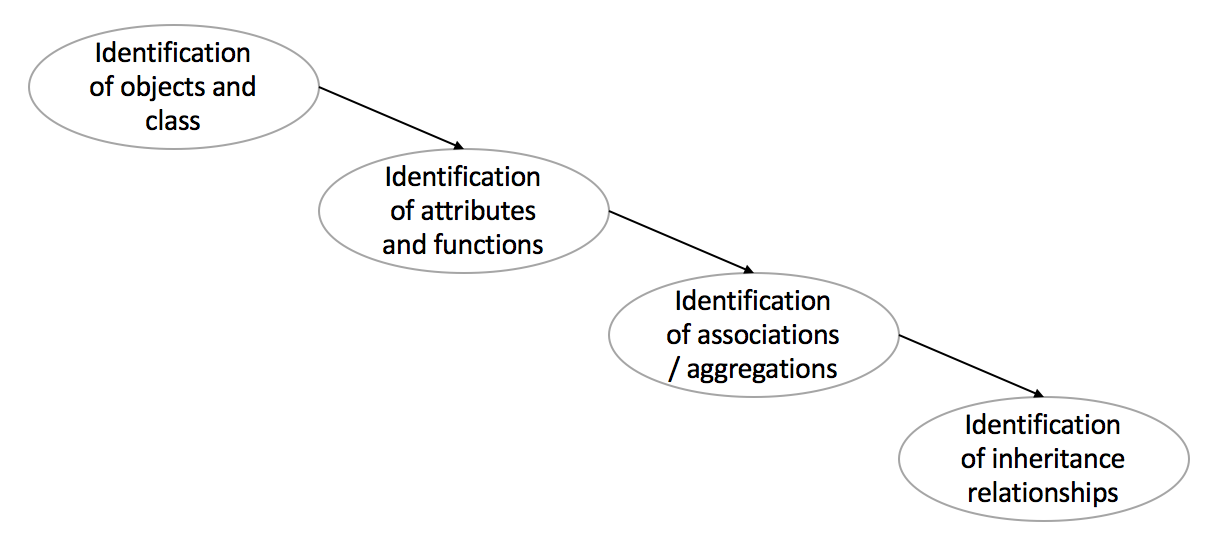
\includegraphics[width=14cm, keepaspectratio]{img/construml}
  \caption{Diagrama de definición de UML}
  \label{fig:construml}
\end{figure}

Las clases en UML son representadas como un rectángulo dividido en nombre de la clase, atributos y operaciones o métodos, tal como podemos ver en la Figura \ref{fig:diagrama-de-clases}.

\begin{figure}[htb]
  \centering
  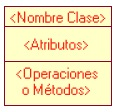
\includegraphics[width=2cm, keepaspectratio]{img/clase1}
  \caption{Representación de clase.}
  \label{fig:diagrama-de-clases}
\end{figure}

\begin{itemize}
  \item Clases: encapsulan la información de un objeto. Pueden ser abstractas si no tienen instancias directas pero sus descendientes si las tienen, o concretas que son todas aquellas clases que pueden ser instanciables.
  \item Atributos: se definen como las características que presenta una clase. Pueden ser \emph{public} representado con cuadro azul, \emph{private} representado con un cuadro azul y un candado o \emph{protected} representado con un cuadro azul y una llave.
  \item Métodos: es la forma en la que el objeto interactúa con el entorno. Pueden ser \emph{public} representado con cuadro rosa, \emph{private} representado con un cuadro rosa y un candado o \emph{protected} representado con un cuadro rosa y una llave.
\end{itemize}
En cuanto a las relaciones entre clases, se representa con flechas y según sea el estilo de la flecha, representa
una relación u otra. En la Figura~\ref{fig:flechasrelacion} podemos observar los distintos tipos que existen y que son:

\begin{itemize}
  \item Herencia: indica que una subclase, incluye los métodos y atributos de la clase superior.
  \item Agregación: para componer objetos complejos en los que no es suficiente con los datos básicos.
  \item Asociación: relación de objetos que colaboran entre sí.
  \item Dependencia o Instanciación: sucede cuando la instancia de un objeto depende de otro objeto.
\end{itemize}

\begin{figure}[htb]
  \centering
  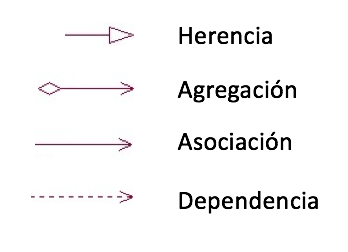
\includegraphics[width=5cm, keepaspectratio]{img/flechasrelacion}
  \caption{Estilos de flechas de relación}
  \label{fig:flechasrelacion}
\end{figure}

\subsection{¿Cómo crear un diagrama de clases?}
\label{subsec:creardiagrama}
Los archivos de UML se suelen presentar en formato imagen o con la extensión xmi. En la Figura~\ref{fig:ejemplouml} podemos ver un ejemplo sencillo de un diagrama UML presentado en formato imagen y en el listado~\ref{lst:ejemploxmi} podemos ver el formato que se presenta en los archivos xmi, para generar los diagramas.

\begin{figure}[htb]
  \centering
  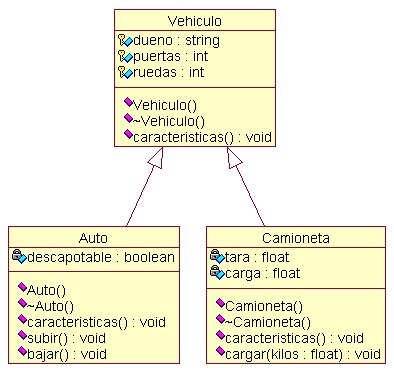
\includegraphics[width=8cm, keepaspectratio]{img/ejemplouml}
  \caption{Ejemplo de una representación de un diagrama de clases de UML}
  \label{fig:ejemplouml}
\end{figure}

Para el caso de la Figura~\ref{fig:ejemplouml} se observa que hay tres clases, en las que \textit{Auto} y \textit{Camioneta} heredan de \textit{Vehículo}. Por explicar uno de ellos, nos centramos en la primera caja (clase) la cual se compone de:

\begin{itemize}
  \item \textbf{Nombre de la clase:} Vehículo.
  \item \textbf{Atributos:} dueño, puertas y rueda. Estos atributos están acompañados de un icono de una llave con cuadro azul, esto significa que es \textit{Protected}, por lo tanto no son visibles desde fuera de la clase pero podrán ser usados por métodos y por las subclases heredadas.
  \item \textbf{Métodos:} Vehículo() y Características(). Estos métodos están acompañados de un icono de un cuadro rosa, esto significa que es \textit{Public}, por lo tanto son visibles desde dentro y fuera de la clase.
\end{itemize}

Las clases \textit{Auto} y \textit{Camioneta} tienen los atributos y métodos de Vehículo, además de sus atributos y métodos particulares.

\begin{lstlisting}[caption={Ejemplo de una clase en un archivo xmi},label={lst:ejemploxmi},breaklines=true, basicstyle=\small]
<UML:Class visibility=``public'' isSpecification=``false'' namespace=``Logical View'' isAbstract=``false'' isLeaf=``false'' isRoot=``false'' xmi.id=``n0m23KIFJiLQ'' name=``Pokemon''>
       <UML:Classifier.feature>
        ...
        <UML:Attribute visibility=``private'' isSpecification=``false'' xmi.id=``w6TDmoeRlXg3'' type=``35BlKE3lbriZ'' name=``level''/>
        ...
        <UML:Operation visibility=``public'' isSpecification=``false'' isQuery=``false'' isAbstract=``false'' isLeaf=``false'' isRoot=``false'' xmi.id=``fm0T9HHMAtpO'' name=``print_ataques_pokemon''/>
       </UML:Classifier.feature>
</UML:Class>
\end{lstlisting}

Para el caso de el Listado~\ref{lst:ejemploxmi}, se observa cómo se escriben estos diagramas en archivos .xmi. El código se ha obtenido a partir de uno de los proyectos analizados, y se ha simplificado eliminando elementos no relevantes, de manera que sea más fácil observar los elementos deseados:

\begin{itemize}
   \item \textbf{Nombre de la clase:} Pokemon. El nombre de la clase lo podemos observar en la etiqueta UML:Class, indicado el nombre en el atributo \emph{name}.
   \item \textbf{Atributos:} \emph{level}. Para este caso, tenemos que buscar las etiquetas UML:Attribute que estén encerradas dentro de la etiqueta UML:Class, indicado el nombre en el atributo \emph{name}. También podemos observar que es un atributo privado, tal como indica en \textit{visibility=private}.
   \item \textbf{Métodos:} print\_ataques\_pokemon. Para este caso, tenemos que buscar las etiquetas UML:Operation que estén encerradas dentro de la etiqueta UML:Class, indicado el nombre en el atributo \emph{name}. También podemos observar que es un método público, tal como indica en \textit{visibility=public}.
\end{itemize}

Para poder generar los diagramas se usan programas externos, que a partir de diseños gráficos de diagramas, se realiza ingeniería inversa para poder exportar en archivos .xmi. Hay una gran lista de programas, tanto gratuitos como de pago, que facilitan esta labor.

\section{Tecnologías de Servidor}
\label{sec:seccion2}

\subsection{Django}
\label{subsec:django}
\textbf{Django}\footnote{https://www.djangoproject.com/} es un framework de software libre de desarrollo web para crear aplicaciones Web de alta calidad
disminuyendo código, basado en DRY (Don't Repite Yourself)~\cite{forcier2008python}. Surgió debido a las necesidades de la aplicación
de noticias de la World Company.

Se aproxima al patrón de diseño MVC (Modelo-Vista-Controlador), en el cual se separa
el acceso y definición de datos (Modelo), de la asignación de ruta lógica (Controlador) y
de la interfaz de usuario (Vista). En la Figura~\ref{fig:esquemadjango} podemos observar el esquema de funcionamiento.

\begin{figure}[htb]
  \centering
  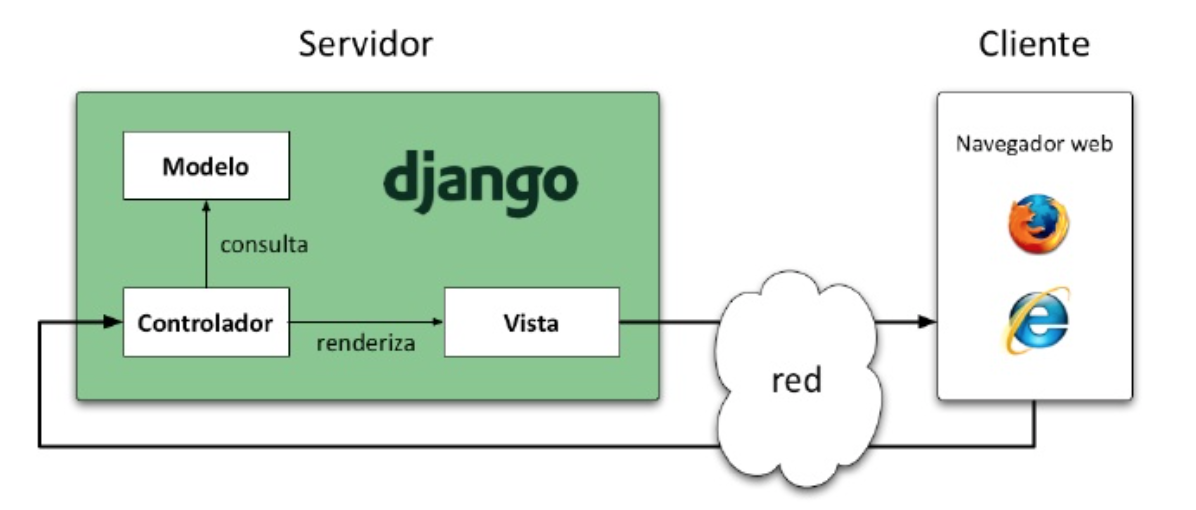
\includegraphics[width=12cm, keepaspectratio]{img/esquemadjango}
  \caption{Esquema de funcionamiento general de un servidor Django}
  \label{fig:esquemadjango}
\end{figure}

El navegador realiza una petición al servidor, mediante la solicitud de una URL, la cual llega al controlador. Desde el controlador se consulta la vista asociada a esa URL, en el archivo urls.py, y cuando se encuentra se  llama a la vista en el archivo views.py. Desde esa vista se consulta la base de datos, el \emph{modelo} en el \emph{argot} de Django, si fuera necesario. Una vez generada la vista, se \emph{renderiza} la página web y se envía al navegador mediante el protocolo HTTP.

Este patrón de diseño favorece la creación de páginas web dinámicas de manera sencilla e independiente, de manera que en caso de
modificación de un componente, este no afecte a otro, es decir, tiene un acoplamiento débil.

Debido a las cualidades que tiene Django, se decide utilizar para la creación de la parte \emph{front-end} del proyecto, la página web de presentación de resultados. La justificación de la elección de Django es porque tenemos que dar resultados de distintos proyectos, tarea que facilita Django con el MVC, al cual se le pasan los datos obtenidos en la consulta de la base de datos a la plantilla, y Django ya crea el HTML resultante.
Otra causa de la elección de Django para este proyecto, es porque el desarrollo de la herramienta ha sido en Python, y Django es un framework en Python.

\subsection{Exuberant Ctags}
\label{subsec:ctags}
\textbf{Exuberant ctags}\footnote{http://ctags.sourceforge.net} es una variante extendida de ctags, que es una herramienta de programación que genera un archivo de etiquetas en texto plano a partir
del código fuente de un programa~\cite{hiebert1999exuberant}. En el archivo de etiquetas se indican funciones,
variables, clases, macros... dependiendo del lenguaje de programación.
Actualmente soporta 41 lenguajes de programación, pero nosotros vamos a centrarnos en Python como prueba de concepto.

Normalmente es utilizada para la localización de las definiciones o tipos, por numerosos editores de código o entornos de desarrollo integrados (IDEs por sus siglas en inglés) y otras utilidades.

A continuación se muestra el ejemplo de fichero ctags obtenido en un proyecto analizado:

\begin{lstlisting}[basicstyle=\small, breaklines=true]
  !_TAG_FILE_FORMAT	2	/extended format; --format=1 will not append ;" to lines/
  !_TAG_FILE_SORTED	1	/0=unsorted, 1=sorted, 2=foldcase/
  !_TAG_PROGRAM_AUTHOR	Darren Hiebert	/dhiebert@users.sourceforge.net/
  !_TAG_PROGRAM_NAME	Exuberant Ctags	//
  !_TAG_PROGRAM_URL	http://ctags.sourceforge.net	/official site/
  !_TAG_PROGRAM_VERSION	5.8	//
  GamePresentation	GamePresentation.py	/^class GamePresentation:$/;"	c
  display	GamePresentation.py	/^    def display(self, message):$/;"	m	class:GamePresentation
  get_choice	GamePresentation.py	/^    def get_choice(self, options):$/;"	m	class:GamePresentation
\end{lstlisting}

\begin{itemize}
  \item Las seis primeras líneas corresponden a información generada por Exuberant Ctags.
  \item Las tres últimas corresponden al análisis realizado por Exuberant Ctags, explicado línea a línea:
  \begin{enumerate}
    \item Por el identificador del final, c, sabemos que es una clase, y el nombre lo podemos extraer del principio de la línea.
    \item Por el identificador del final, m, sabemos que es un método correspondiente a la clase GamePresentation, llamado display tal como podemos ver al principio de la línea.
    \item Por el identificador del final, m, sabemos que es un método correspondiente a la clase GamePresentation, llamado get\_choice tal como podemos ver al principio de la línea.
  \end{enumerate}
\end{itemize}

Se ha utilizado Exuberant Ctags para poder analizar los archivos de código fuente en lenguaje Python, mediante este análisis se extraían los nombres de las clases de todos los ficheros en lenguaje Python disponibles.


\subsection{Python}
\label{subsec:python}
\textbf{Python}\footnote{https://www.python.org} es un lenguaje de programación, creado a finales de los años 80 del siglo pasado, caracterizado
por la legibilidad del código~\cite{van2003python,summerfield2010programming}. Se caracteriza por ser:
\begin{enumerate}
  \item Interpretado: no necesita de un compilador para ser ejecutados, sino de un interprete. El interprete
  ejecuta el programa directamente, no genera un ejecutable.
  \item De alto nivel: sintaxis sencilla para la comprensión humana.
  \item Multiplataforma: para diversos Sistemas Operativos.
  \item De tipado dinámico: no es necesario declarar el tipo de variable, ya que se asigna
  automáticamente en tiempo de ejecución.
  \item Multiparadigma: permite distintas técnicas de programación (Orientación a objetos, funcional...)
\end{enumerate}

Se decide usar este lenguaje de programación debido a las características que presenta como que es de alto nivel y facilita su compresión, y porque es el lenguaje que más me ha gustado en los años de universidad. Con Python se ha desarrollado todo el proyecto, tanto el servidor con Django como toda la lógica de la herramienta para analizar el código fuente y su modelado UML.

\subsection{API de GitHub}
\label{subsec:apigithub}
\textbf{GitHub}\footnote{https://github.com} es una plataforma para almacenar repositorios, utilizando el control de versiones de Git (ver sección~\ref{subsec:git}), en la que destaca el desarrollo colaborativo. Ofrece, además de los repositorios git, funcionalidades como un sistema de gestión de erratas, wikis, una web pública y la posibilidad de que hacer ramificaciones (\emph{forks}) de un repositorio.

La API de GitHub ofrece distintas funcionalidades para obtener datos sobre los más de 45 millones de repositorios alojados en GitHub. En nuestro caso vamos a usar la API que da información sobre los repositorios:

  \begin{lstlisting}
    GET https://api.github.com/repos/user/project
  \end{lstlisting}

Así, para los proyectos que nos interesen, realizaremos una petición HTTP siguiendo el interfaz indicado en la API. Si el proyecto existe, recibiremos una respuesta HTTP con un \emph{200 OK} y un fichero/objeto JSON con los datos. Si no existe el proyecto, la cabecera HTTP será \emph{404 Not Found} y el objeto JSON contendrá un mensaje de error.

Otro uso que se le ha dado a GitHub ha sido para almacenar el proyecto\footnote{https://github.com/calvarezpe/WebPage-UML} lo que permite hacer pública la herramienta desarrollada, permite colaboración de otros programadores y mantener un control de versiones, estando disponible la versión que más nos interese. En otro repositorio se ha almacenado la memoria del proyecto, con el principal objetivo del control de versiones.

\subsection{Git}
\label{subsec:git}

Git es un sistema de control de versiones gratuito y de código abierto diseñado para gestionar los diversos cambios que se realizan a lo largo del desarrollo de un proyecto. De esta manera, se puede restaurar a versiones anteriores en caso de que se produzcan fallos o por alguna razón se quiera recuperar el estado anterior.
Permite la realización de un trabajo en equipo de manera eficiente y rápida. Destaca por que los cambios se importan como ramas diferentes a la principal, y pueden ser fusionadas a esta en el momento que se decida.

A continuación se muestran comandos básicos de \textit{supervivencia}~\cite{sanchez2016git}.

\begin{lstlisting}[breaklines=true, basicstyle=\small]
  git init ## Para crear un nuevo repositorio Git
  git clone <<url_repo>> ## Para crear una copia local de un repositorio
  git add <<filename>> ## Para añadir un archivo al repositorio Git
  git commit -m "message" ## Para registrar los cambios
  git push ## Para enviar los cambios al servidor
  git pull ## Para actualizar el repositorio local
  git status ## Información de estado de los ficheros del repositorio
\end{lstlisting}

Se decide usar Git porque es la herramienta de control de versiones más conocida y usada, lo cual nos interesa ya que nuestra herramienta desarrollada se trata de un piloto en desarrollo, y todas las aportaciones realizadas serán de utilidad para ello. También se decide usar Git ya que es la herramienta de control de versiones utilizada en la universidad.

\section{Tecnologías en el Cliente}
\label{sec:seccion3}

\subsection{HTML5}
\label{subsec:html5}

HTML5 es la quinta versión de \textbf{HTML} (HyperText Markup Language), lanzada en 2014~\cite{pilgrim2010html5,gauchat2012gran}. Se trata de un lenguaje de marcado para la realizar páginas web de manera
estructurada. Se incluyen nuevos elementos, atributos y comportamientos. También incluye más tecnologías
que permiten a las páginas webs ser mas diversas y atractivas, soportado por la mayoría de navegadores.

Cuenta con numerosas etiquetas para contenido multimedia, que lo hace interesante debido a
que no es necesario el uso de Flash, ni de instalar nada de forma adicional. Además, y como gran novedad respecto a versiones anteriores del mismo estándar, provee con una serie de interfaces (APIs) para JavaScript, permitiendo la creación de aplicaciones web con HTML5 que compitan con aplicaciones de escritorio, con todas las consecuencias de desarrollo y de uso que esto acarrea.

En este proyecto se ha utilizado HTML5 para las páginas webs presentadas al usuario a través del sistema de plantillas de Django, es decir, las plantillas utilizadas en Django son en HTML5. Tiene la ventaja que presenta una velocidad de carga rápida, lo cual nos beneficia, ya que el análisis del proyecto puede llevar más tiempo y la carga de la página no nos penaliza en tiempo.

\subsection{CSS3}
\label{subsec:CSS3}

\textbf{CSS3} (Cascading StyleSheets) es la última evolución de las hojas de estilo en cascada CSS, que es un lenguaje de diseño gráfico para la presentación de documentos
definidos en HTML~\cite{mcfarland2012css3,gauchat2012gran}. Es la mejor forma para separar contenidos y su presentación.
El W3C apostó por el desarrollo y estandarización de CSS y en 1996 publicó la primera recomendación.

Con HTML se marcan los contenidos de la página, y se utiliza CSS para definir el aspecto de cada
elemento marcado, como tamaño, color, tipo, separación...

CSS3 incorpora muchas novedades muy esperadas como esquinas redondeadas, sombras, animaciones, nuevos \emph{layouts}...
Las partes experimentales son especiales para cada navegador, y no es recomendable su uso en producción.

Se utiliza CSS porque nos permite tener separado los detalles de como mostrarlo a la información del contenido a mostrar. Se utiliza en el diseño de la página web mostrada al usuario, para que esta tenga un buen aspecto y sea intuitiva.
\subsection{JavaScript}
\label{subsec:javascript}

JavaScript es un lenguaje de programación ligero e interpretado~\cite{flanagan2006javascript,gauchat2012gran}. Su uso principal es en páginas web pero también se usa en otros entornos.
Surgió la necesidad, en los años 90, la creación de un nuevo lenguaje de programación debido a la creación de las aplicaciones webs. El problema que se planteaba con las aplicaciones webs en esa fecha era la baja velocidad que los usuarios tenían en internet, de manera que para poder ofrecer aplicaciones webs sin esperar mucho tiempo, surgió la necesidad de un lenguaje de programación que se ejecutase en el navegador del usuario, y no en un servidor como era usual.

JavaScript se caracteriza por ser orientado a objetos, basado en prototipos, imperativo, débilmente tipado y dinámico.

En nuestra página web, se utiliza JavaScript para comprobar la URL que introduce el usuario, de manera que no tiene que esperar a que el servidor le de una respuesta si la URL está bien estructurada o no, es decir, si presenta el formato general de una URL.

\subsection{BootStrap}
\label{subsec:bootstrap}
\textbf{BootStrap}\footnote{http://getbootstrap.com} es un framework desarrollado y liberado por Twitter~\cite{cochran2012twitter}. Surge a raíz de la multitud de ingenieros trabajando en Twitter por el mismo proyecto, para utilizar todos el mismo framework. Se lanzó de manera pública en agosto de 2011, en la plataforma GitHub, pero debido a su potencial, numerosos programadores empezaron a colaborar sobre este proyecto, convirtiéndolo en el proyecto de software libre más activo del mundo.

BootStrap se trata de una colección de elementos web personalizables y funciones en una única herramienta. Su principal objetivo es facilitar el diseño web, basándose en una combinación de HTML, CSS y JavaScript. Se encuentra en continuo desarrollo gracias a ser software libre.

Se puede hacer uso de varias formas, pero nosotros lo haremos a través de la CDN de BootStrap incluyendo el siguiente código en nuestro archivo HTML:

  \begin{lstlisting}[basicstyle=\small, language=HTML, breaklines=true]
    <link rel=``stylesheet'' href=``//netdna.bootstrapcdn.com/bootstrap/3.1.0/css/bootstrap.min.css''>
    <script src=``//netdna.bootstrapcdn.com/bootstrap/3.1.0/js/bootstrap.min.js''></script>
  \end{lstlisting}

BootStrap facilita la creación de páginas webs sencillas con interfaces limpias para el usuario y de manera \emph{responsive}, es decir, que se adapta a todo tipo de dispositivos. Es compatible con la mayoría de navegadores actuales.

Se ha utilizado BootStrap en las tres vistas disponibles de la página web:
\begin{itemize}
  \item Página principal, en la cual se han utilizado el estilo de botón, el estilo de letra y el estilo de caja input.
  \item Página para mostrar resultados (de uno o varios proyectos), en el cual se ha utilizado el estilo completo de tabla mediante el cual con una simple línea de código se obtiene una tabla \emph{responsive}, la cual señala el elemento al pasar por encima el ratón, y muestra cada elemento de un color. La línea introducida ha sido la siguiente:
  \begin{lstlisting}[basicstyle=\small, language=HTML, breaklines=true]
    <table class="table table-striped table-bordered table-hover table-condensed">
  \end{lstlisting}
\end{itemize}

En definitiva, se consiguen muy buenos resultados de manera muy sencilla.

%%%%%%%%%%%%%%%%%%%%%%%%%%%%%%%%%%%%%%%%%%%%%%%%%%%%%%%%%%%%%%%%%%%%%%%%%%%%%%%%
%%%%%%%%%%%%%%%%%%%%%%%%%%%%%%%%%%%%%%%%%%%%%%%%%%%%%%%%%%%%%%%%%%%%%%%%%%%%%%%%
% DISEÑO E IMPLEMENTACIÓN %
%%%%%%%%%%%%%%%%%%%%%%%%%%%%%%%%%%%%%%%%%%%%%%%%%%%%%%%%%%%%%%%%%%%%%%%%%%%%%%%%

\cleardoublepage
\chapter{Diseño e implementación}

En este capítulo se muestra la arquitectura de la aplicación web,
el acoplamiento entre los componentes y la especificación de cada parte de la aplicación.

\section{Arquitectura general}
\label{sec:arquitectura}

La aplicación consta de parte servidora, que es donde se lleva a cabo toda la lógica, y
la parte cliente, que es donde se muestran los resultados obtenidos. En la Figura~\ref{fig:arquitectura}
podemos ver el esquema general, indicando para cada módulo las tecnologías que se usan.
\begin{figure}[htb]
  \centering
  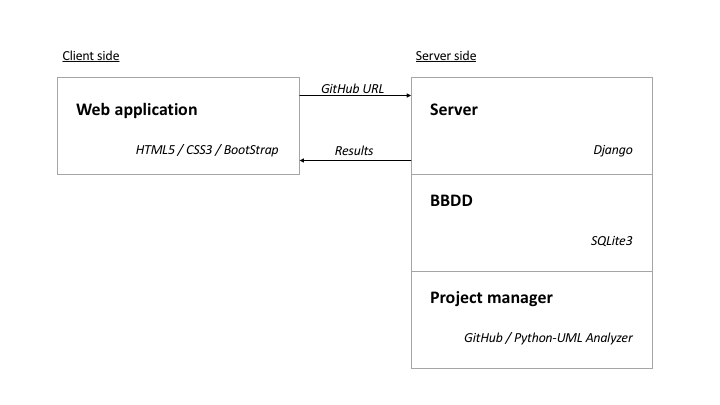
\includegraphics[width=12cm, keepaspectratio]{img/arquitectura-web}
  \caption{Arquitectura aplicación web}
  \label{fig:arquitectura}
\end{figure}

Debido a la configuración de la página web, se pueden solicitar dos opciones: analizar un proyecto
dada su página web en GitHub o consultar todos los proyectos disponibles en la base de datos. Se considera proyecto
disponible todo aquel que haya sido analizado anteriormente.


\begin{itemize}
  \item \textbf{Analizar un proyecto dada su página web en GitHub.} En este caso, si el proyecto existe
  en GitHub, el resultado será de una nueva página con una tabla indicando los resultados que se obtienen
  para dicho proyecto. Los resultados que se muestran son el número de clases en UML, el número de clases en Python,
  la intersección entre ambas y su porcentaje, y un desglose de la intersección. En la Figura~\ref{fig:flujoweb} podemos observar el diagrama de flujo de la web.
  \item \textbf{Consulta de todos los proyectos.} Cuando se selecciona esta opción, se mostrará una nueva página
  con un estilo similar a la tabla anterior, pero mostrando todos los proyectos analizados anteriormente y se encuentren
  en la base de datos de la aplicación.
\end{itemize}

\begin{figure}[htb]
  \centering
  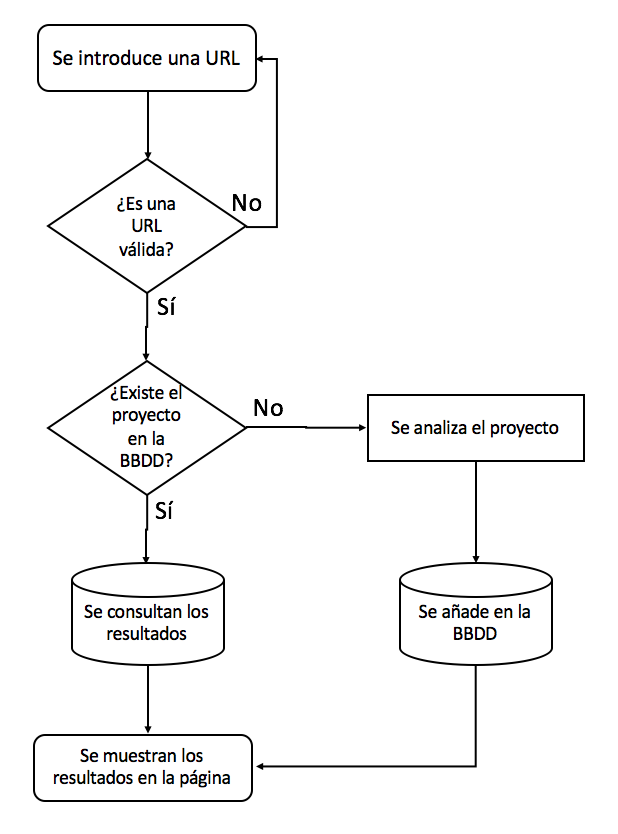
\includegraphics[width=9cm, keepaspectratio]{img/flujoweb}
  \caption{Flujo de interacción de la web.}
  \label{fig:flujoweb}
\end{figure}

Es necesario entender el funcionamiento de cada módulo, detallado a continuación.

\subsection{Cliente (Front-end)}
\label{subsec:cliente}
\subsubsection{Frontal página web}
\label{subsubsec:frontweb}
El frontal de la página web, es la parte que ve el cliente. Se apuesta por un modelo sencillo
y claro, que no permita dudas al uso, tal como observamos en la Figura~\ref{fig:mainpage}

\begin{figure}[htb]
  \centering
  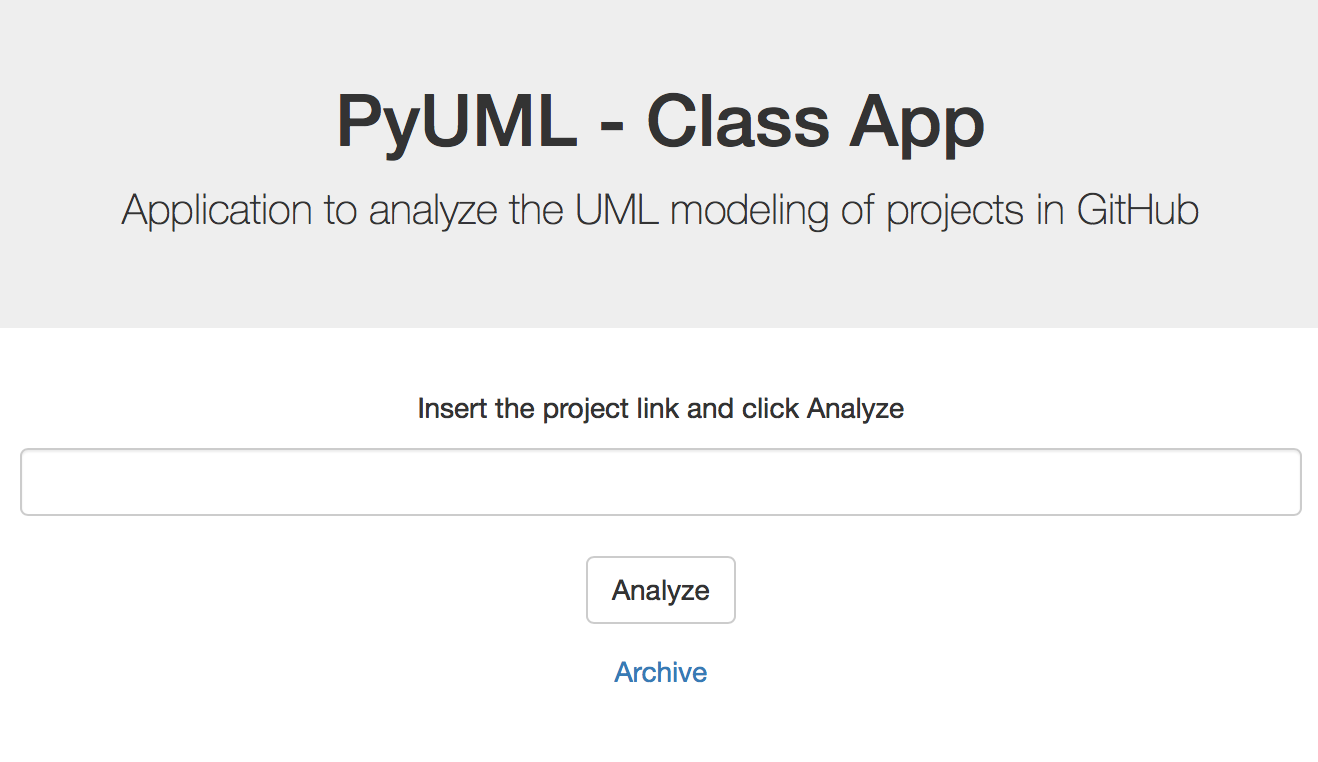
\includegraphics[width=10cm, keepaspectratio]{img/mainpage}
  \caption{Página principal de la aplicación web.}
  \label{fig:mainpage}
\end{figure}

Se muestra un cuadro en el cual se debe ingresar la página web donde está alojado el repositorio de GitHub,
un botón para proceder al envío de la URL y un enlace para consultar los proyectos disponibles.
El método de envío del formulario es mediante un método HTTP POST, ya que permite que los datos enviados no sean visibles al usuario,
y no lleguen datos inesperados a nuestro servidor.

Tras ingresar el enlace de un proyecto válido en GitHub, se muestran los resultados para dicho proyecto. La Figura~\ref{fig:resultsproject} muestra un ejemplo.
\begin{figure}[htb]
  \centering
  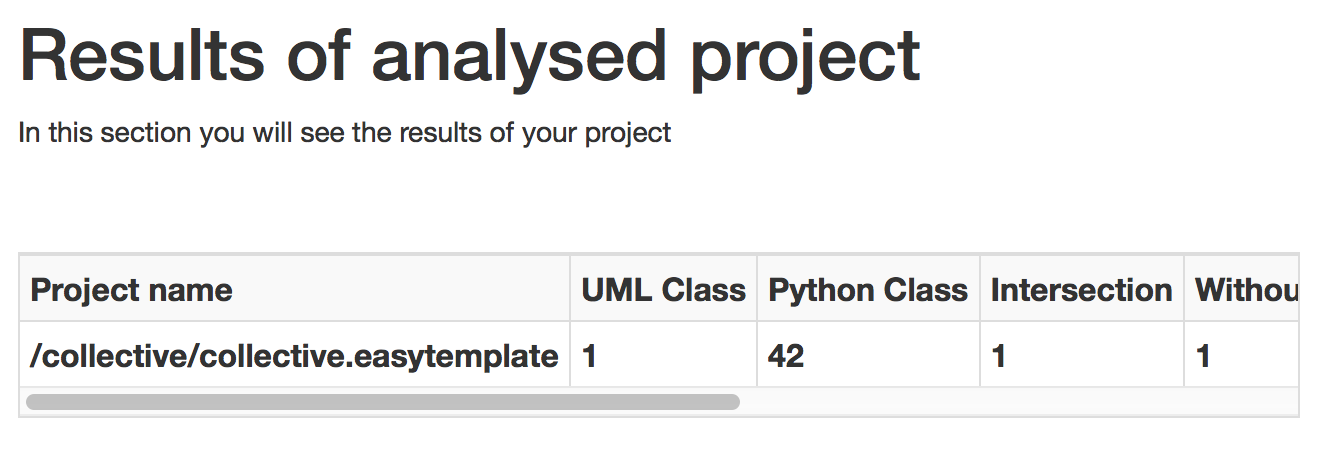
\includegraphics[width=10cm, keepaspectratio]{img/resultsproject}
  \caption{Ejemplo de resultados de un proyecto.}
  \label{fig:resultsproject}
\end{figure}

Otra opción de la página, es la consulta de los proyectos analizados hasta el momento. La vista de resultados se trata de una tabla, formada por todos los resultados de todos los proyectos, tal como muestra la Figura~\ref{fig:archive}
\begin{figure}[htb]
  \centering
  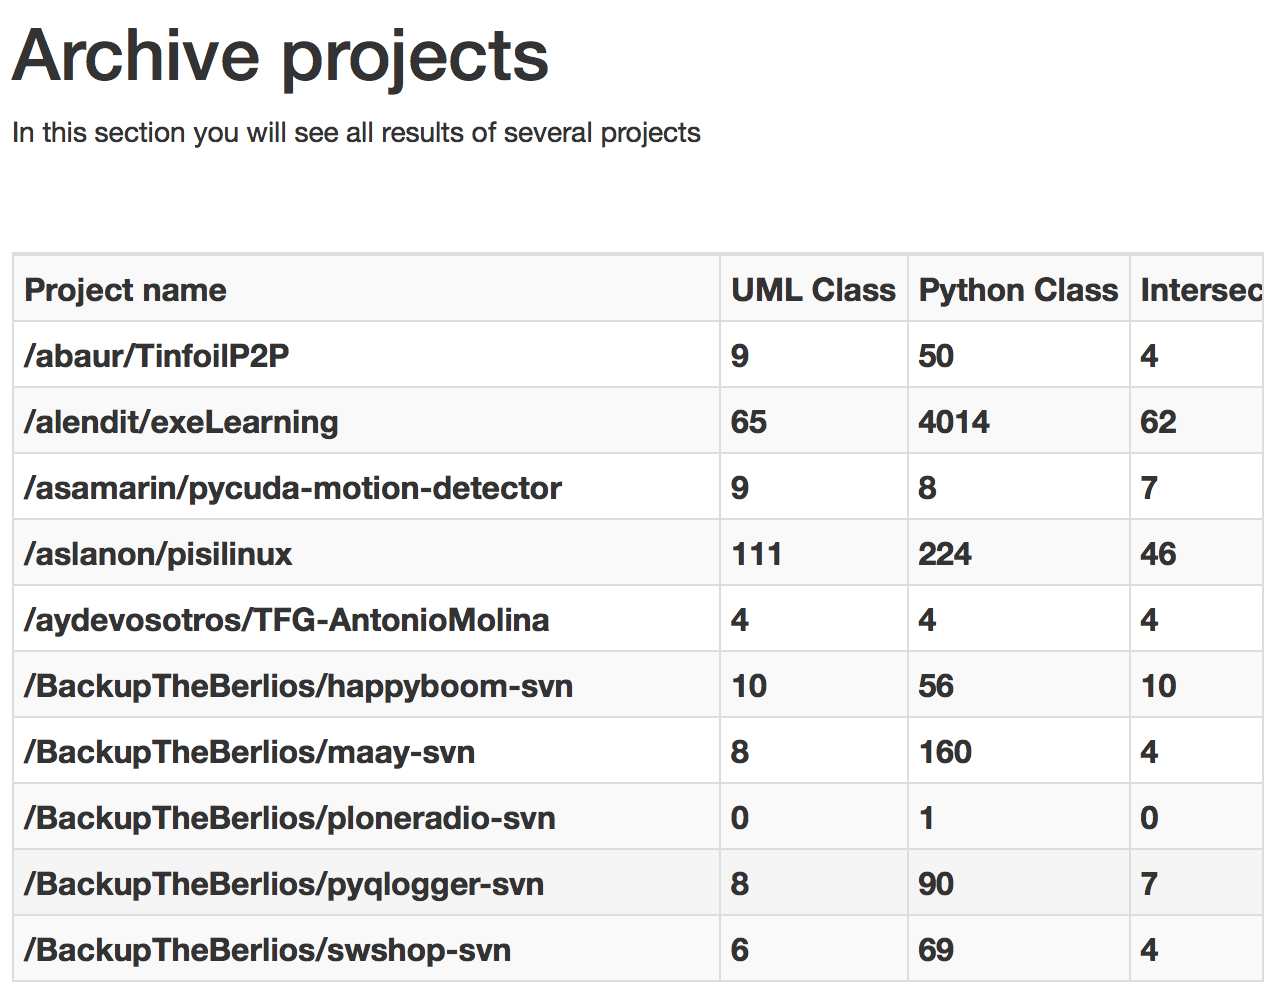
\includegraphics[width=10cm, keepaspectratio]{img/archive}
  \caption{Vista de la página Archive.}
  \label{fig:archive}
\end{figure}

\subsection{Servidor (Back-end)}
\label{subsec:servidor}
\subsubsection{Servidor Django}
\label{subsubsec:server}
El servidor Django necesita de distintos archivos para poder funcionar. A continuación se muestra la estructura
completa:

\begin{figure}[htb]
  \centering
  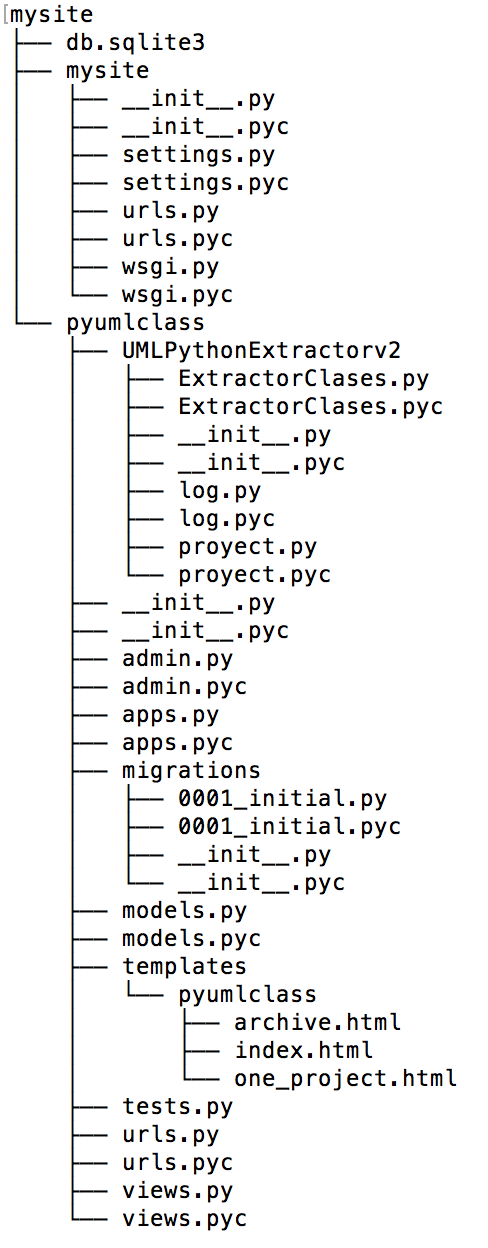
\includegraphics[width=4cm, keepaspectratio]{img/estructura-server}
  \caption{Estructura de ficheros en el servidor}
  \label{fig:estructura-server}
\end{figure}

Tal como se puede observar en la Figura~\ref{fig:estructura-server}, el directorio raíz
está formado por:
\begin{itemize}
  \item \textbf{db.sqlite3} que es el archivo de la base de datos.
  \item \textbf{manage.py} que sirve para interactuar con Django a través de comandos en el terminal.
  \item \textbf{mysite} que es el directorio principal del servidor Django. Dentro de este directorio,
  los archivos que usamos son \textit{urls.py}, en el cual tenemos que incluir todas las
  URLs de nuestra aplicación y \textit{settings.py}, en el cual disponemos de la configuración general del servidor,
  en el cual tenemos que indicar la existencia de nuestra aplicación, la base de datos a utilizar, el huso horario...
  \item \textbf{pyumlclass} que es el directorio donde está toda la lógica de nuestra aplicación. Es necesario realizar
  una explicación de los siguientes archivos/directorios:
  \begin{itemize}
    \item \textbf{UMLPythonExtractorv2} es el directorio donde se encuentra todo el código necesario para analizar
    el código Python y UML, no vamos a entrar en detalle en este apartado ya que será explicado en el módulo Analizador
    Python-UML.
    \item \textbf{models.py} en este archivo se encuentran los modelos (objetos) necesarios que hará uso nuestra aplicación.
    Para nuestro caso, se ha creado un único modelo llamado \emph{Project}, y con las propiedades necesarias para mostrar los
    datos en nuestra aplicación. Podemos ver más detalle en la Figura~\ref{fig:project-model}
    \begin{figure}[htb]
      \centering
      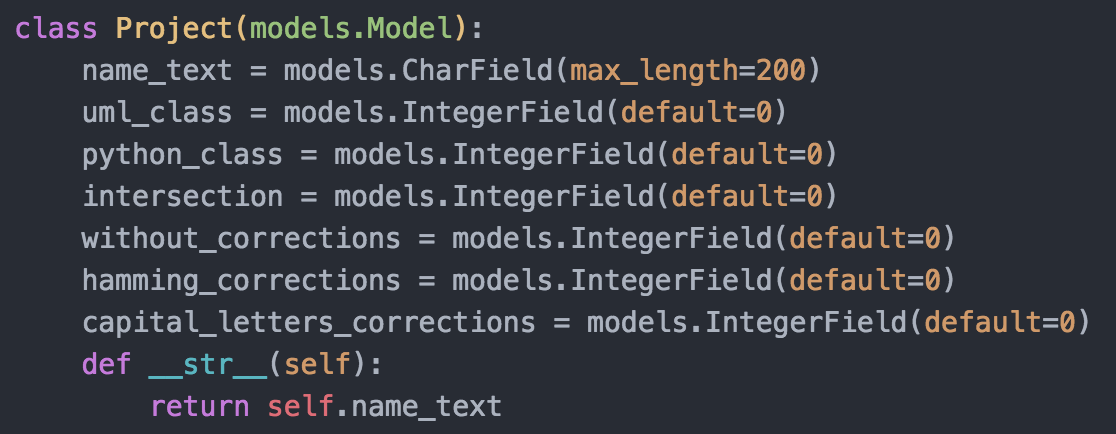
\includegraphics[width=12cm, keepaspectratio]{img/project-model}
      \caption{Modelo para nuestra aplicación}
      \label{fig:project-model}
    \end{figure}
    \item \textbf{templates} es el directorio donde se almacenan las plantillas HTML de nuestra web.
    \item \textbf{urls.py} es el archivo denominado controlador en el cual se indica la vista
    que se mostrará en el momento que se pida una URL. Django utiliza un conjunto de patrones que intentará
    hacer coincidir la dirección URL recibida con la vista correcta. En la Figura~\ref{fig:controlador-urls} podemos observar las URLs disponibles para nuestra aplicación.
    \begin{figure}[htb]
      \centering
      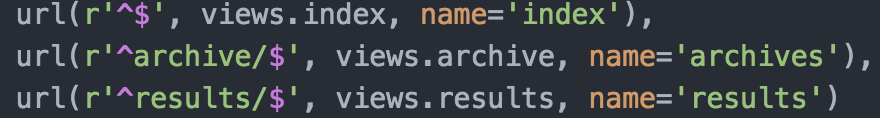
\includegraphics[width=10cm, keepaspectratio]{img/controlador-urls}
      \caption{URLs del controlador}
      \label{fig:controlador-urls}
    \end{figure}

    Vamos a proceder a explicar el último caso de la Figura~\ref{fig:controlador-urls}. El primer operando sirve para especificar la URL
    a la que queremos asociar, en este caso \textit{results}, sera asociada a la vista \emph{results} ubicada en views.results.
    \item \textbf{views.py} es el archivo donde se encuentran las vistas de nuestro servidor. Existe una vista por cada
    página disponible de nuestro servidor, por lo tanto en nuestro caso hay 3: para la página principal, para la página
    de archivo donde se encuentran todos los resultados de los proyectos y la página de resultados a partir de una URL
    dada.

  \end{itemize}
\end{itemize}

Por lo tanto el proceso sería, el servidor Django recibe una URL, el controlador buscará cual es la vista correcta
para esa URL, y en caso de éxito, llamaría a la vista. La vista realizaría todo lo que este indicado en sí para cada caso,
y respondería renderizando la plantilla HTML.

\subsubsection{Base de datos SQLite3}
\label{subsubsec:bbdd}

SQLite3 es una base de datos relacional, que viene por defecto en Django~\cite{owens2010sqlite}.
En la base de datos almacenamos nombre del proyecto, número de clases de UML,
número de clases de Python, intersección de clases, número de clases sin corrección, número de clases
corregidas por errores de mayúsculas y número de clases corregidas por errores en distancia de Hamming.


\subsubsection{GitHub}
\label{subsubsec:github}
Se realiza una descarga del repositorio para poder realizar el análisis del proyecto. La descarga
se hace ejecutando el siguiente código:

\begin{figure}[htb]
  \centering
  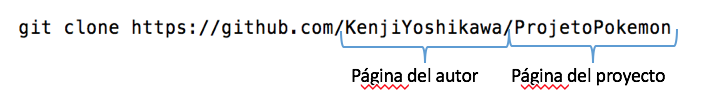
\includegraphics[width=12cm, keepaspectratio]{img/codigo-git}
  \caption{Instrucción para descargar un proyecto desde GitHub}
  \label{fig:codigogit}
\end{figure}

Esto crea una carpeta en el directorio donde se haya ejecutado el código con el nombre que aparezca
en GitHub como nombre del proyecto.

\subsubsection{Analizador Python-UML}
\label{subsubsec:analizadorpyuml}
Este es el módulo principal en el que se basa esta aplicación web, dónde se encuentra toda la lógica. Se muestra el diagrama de flujo en la Figura~\ref{fig:flujoanalizador}.

\begin{figure}[htb]
  \centering
  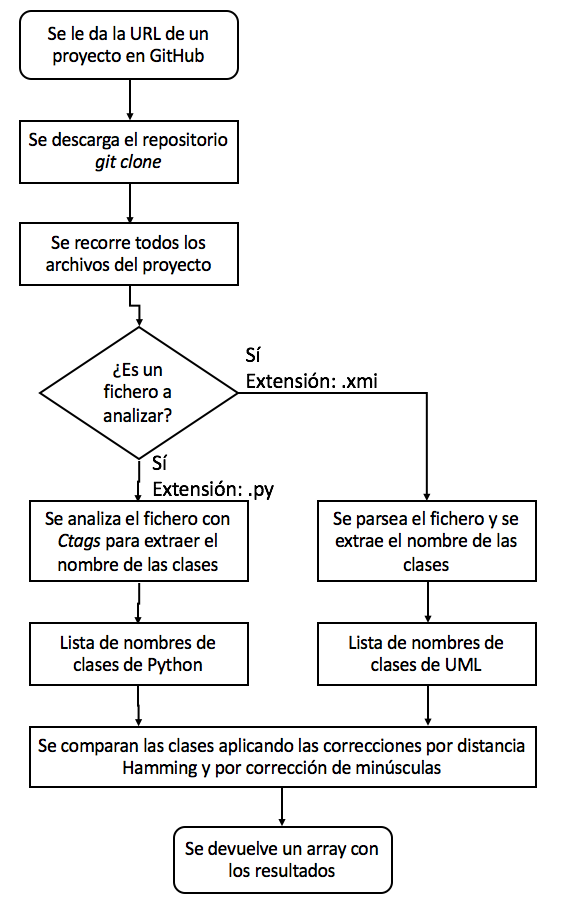
\includegraphics[width=9cm, keepaspectratio]{img/flujoanalizador}
  \caption{Diagrama de flujo del analizador Python-UML}
  \label{fig:flujoanalizador}
\end{figure}

El funcionamiento general de este programa consiste en:
\begin{enumerate}
  \item Como datos de entrada se le tiene que dar una URL de un proyecto almacenado en GitHub. Se descarga
  este proyecto en el directorio local donde se ejecute el programa, para poder analizarlo.
  \item Se recorre todos directorios en busca de archivos UML (.xmi) y Python (.py)
  \item Se extrae el nombre de las clases de los archivos encontrados. Según sea UML o Python se seguirá
  un procedimiento u otro:
  \begin{itemize}
    \item Python. Para la extracción de los nombres de las clases se utiliza Ctags, para ello se ejecuta
    \textit{ctags nombre\_archivo.py}, y Ctags genera un archivo de etiquetas llamado \textit{tags}.

    Este archivo indica en cada linea el tipo que es con atributos o con que está relacionado. Para nuestro
    caso, solo nos fijaremos aquellas que sean marcadas como clases, indicadas con
    una \textbf{c} al final, y nos quedamos con el nombre de la clase.

    Todas las clases de todos los archivos .py serán añadidas a una lista.

    Una vez finalizado este proceso,
    se realiza un proceso de depuración en el que se eliminan duplicados.
    \item UML. Para este caso, se trata el archivo .xmi con un parser, el cual se encarga de extraer las etiquetas. Una vez
    extraídas todas las etiquetas, hay que quedarse únicamente con aquellas consideras UML. Después de esto,
    hay que fijarnos en aquellas marcadas como Clases, y de estas nos quedamos con el nombre de la clase.

    Al igual que en Python, se añaden todas los nombres de las clases de todos los archivos .xmi a una lista, y se
    realiza un proceso de depuración para eliminar duplicados.
  \end{itemize}
  \item Una vez obtenidos todos los nombres de las clases tanto para Python como para UML, se procede a realizar
  un análisis de los nombres obtenidos. Para facilitar las operaciones de análisis, se convierte las listas de clases en \textit{sets},
  que es un tipo de Python definido como colecciones de datos únicos no ordenados. El análisis se divide en tres partes:
  \begin{enumerate}
    \item \textbf{Análisis sin correcciones:} se calcula la intersección existente entre los dos conjuntos. Es decir,
    se crea un \emph{set} nuevo, con los nombres de las clases que tengan en común.

    \begin{figure}[htb]
      \centering
      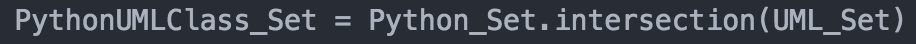
\includegraphics[width=8cm, keepaspectratio]{img/pyumlsets}
      \caption{Código para calcular la intersección}
      \label{fig:pyumlsets}
    \end{figure}

    \item \textbf{Análisis con correcciones por minúsculas:} se convierte las clases en minúsculas y se vuelve a realizar
    la intersección. Se realiza la conversión del resto de clases que aun no han sido emparejadas, para que no haya valores
    a comparar ya añadidos.

    Es decir, el problema que solucionamos con esto es que si una clase en Python se llama `Boss', y en UML se llama `boss', con este método se
    consideran como iguales ya que el concepto `Boss', está representado en UML.

    \item \textbf{Análisis con correcciones por distancia de Hamming:} la distancia de Hamming entre dos palabras es el número
    de letras que tienen diferentes. Es decir, la distancia de Hamming entre \textit{padre} y \textit{madre} es 1.

    Por lo tanto, se consideran equivalentes aquellas clases que presenten fallos por diferencias de tres letras y una
    diferencia de longitud entre ellas menor a 3.

    Por ejemplo, la clase `RBFN', será valida con la clase `RBFNN'.
  \end{enumerate}

  Una vez hechas todas las correcciones, se devuelven los resultados obtenidos:
  \begin{itemize}
    \item Número total de clases.
    \item Número de clases obtenidas sin corregir.
    \item Número de clases obtenidas por corrección de minúsculas.
    \item Número de clases obtenidas por corrección de distancia de Hamming.
    \item Lista de clases de Python que no están representadas en UML.
    \item Lista de clases de UML que no existen en Python.
    \item Lista de clases en común de Python y UML.
  \end{itemize}
  \item Una vez finalizado todo el análisis, se borra la carpeta del proyecto y finaliza el programa.
\end{enumerate}

Para realizar todo este proceso se utiliza tres archivos, de manera que las funciones estén desacopladas
entre sí, y cualquier modificación de una función no afecte a otras.

Para no perder los datos se van almacenando en un fichero .csv\footnote{Un fichero csv es un documento de texto plano en el que se presentan resultados en forma de tabla, de manera que los valores de las columnas están separados por tablas y las filas de nuevos elementos por saltos de línea.}.

%%%%%%%%%%%%%%%%%%%%%%%%%%%%%%%%%%%%%%%%%%%%%%%%%%%%%%%%%%%%%%%%%%%%%%%%%%%%%%%%
%%%%%%%%%%%%%%%%%%%%%%%%%%%%%%%%%%%%%%%%%%%%%%%%%%%%%%%%%%%%%%%%%%%%%%%%%%%%%%%%
% RESULTADOS %
%%%%%%%%%%%%%%%%%%%%%%%%%%%%%%%%%%%%%%%%%%%%%%%%%%%%%%%%%%%%%%%%%%%%%%%%%%%%%%%%

\cleardoublepage
\chapter{Resultados}

Para poder obtener resultados reales, se ha probado la aplicación con varios proyectos de GitHub.
El tutor del proyecto me facilitó una lista de proyectos en GitHub que tienen archivos de UML (verificados por la Universidad de Gotemburgo). Esta lista incluía proyectos con distintos tipos de lenguaje de programación,
y diferentes archivos UML, tal como la extensión .xmi, .uml y en formato imagen. El formato .uml
no se considera estandarizado.

Por lo tanto, del total de esta lista filtramos a aquellos archivos que sean de un proyecto
que use Python, y solo aquéllos que utilicen el formato estándar de UML en archivo, es decir, los
que tienen extensión .xmi. De esta manera, obtenemos 108 proyectos para analizar y poder testear la aplicación.
Estos proyectos nos servirán tanto para entender el uso de UML como para poder optimizar la aplicación
frente a errores que se pudieran dar, al obtener los resultados de tal manera que el proceso y los resultados han sido supervisados y comprobados en todo momento.

Debido a la gran cantidad de datos obtenidos en el análisis, se ha decidido realizar una representación gráfica de los resultados para poder dar una interpretación de los mismos. Los gráficos que se muestran en esta memoria son los siguientes:

\begin{itemize}
  \item Número de clases de UML y de Python de todos los proyectos
  \item Extracto del gráfico anterior del total de proyectos, para poder analizarlos gráficamente
  \item Gráfica que se representa el porcentaje de clases de Python representadas con UML frente al total
  de clases de Python
  \item Gráfica de dos proyectos de ejemplo para interpretar las correcciones realizadas por mayúsculas/minúsculas y
  por distancia de Hamming
\end{itemize}


\section{Análisis total de proyectos}
\label{subsec:analisistotalproyectos}
Se representa gráficamente por cada proyecto las clases de UML y las clases de Python que tienen. De esta manera
podemos ver, \emph{a groso modo}, que la mayoría de clases Python no están representadas en los diagramas UML, sin tener en cuenta
los valores de los nombres de estas clases.

\begin{figure}[htb]
  \centering
  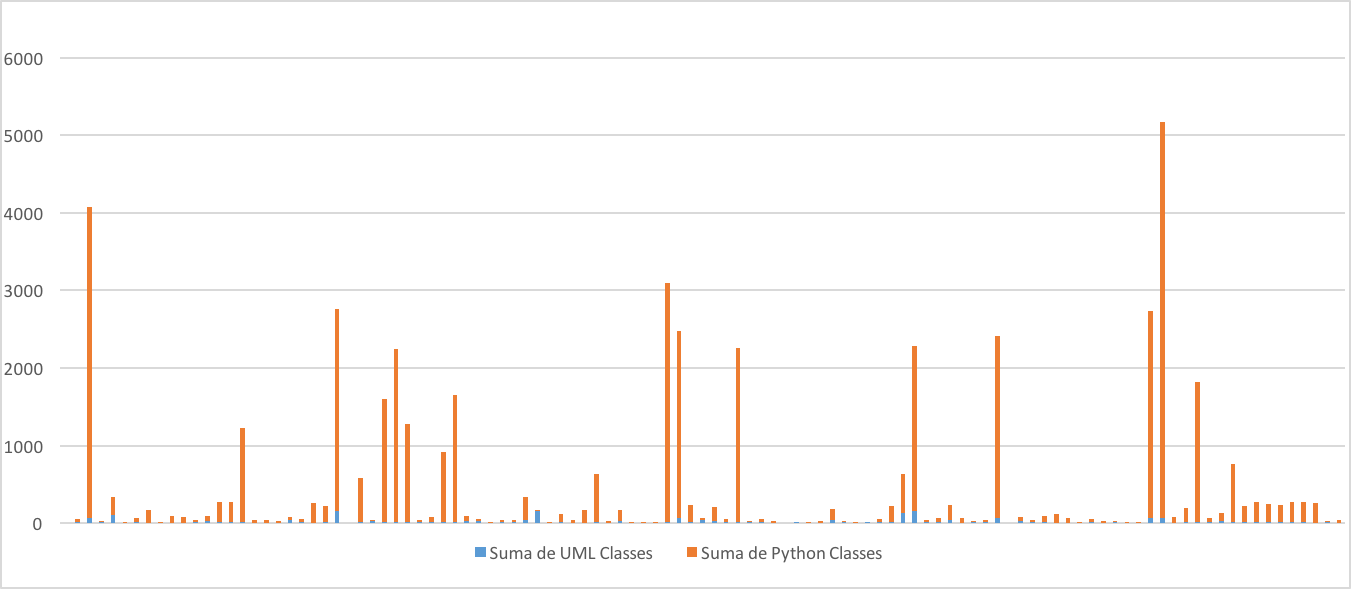
\includegraphics[width=17cm, keepaspectratio]{img/GraficasResultados/todosproyectos}
  \caption{Clases de todos los proyectos}
  \label{fig:totalproyectos}
\end{figure}

Nos encontramos ante un gráfico en el que cada columna representa a un proyecto, y se puede dividir en número de clases en Python y número de clases en UML, siendo cada una representada por un color, naranja y azul respectivamente. En el eje vertical se indica el número de clases de las que dispone el proyecto, siendo las clases de Python y de UML apiladas en una única columna.

Tal como podemos ver en la Figura~\ref{fig:totalproyectos}, el número de clases existentes, para
la mayoría de los proyectos, es superior en Python que en UML.
Hay que tener en cuenta que en esta gráfica sólo se muestra el número de clases de Python y el número
de clases de UML, que no siempre van a ser equivalentes.

Por lo tanto, con esta simple representación, se puede extraer que la mayoría de clases de Python no tienen su equivalente
en UML, o lo que es lo mismo, no están modeladas en UML.


\begin{figure}[htb]
  \centering
  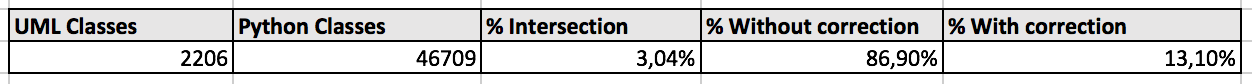
\includegraphics[width=\textwidth, keepaspectratio]{img/GraficasResultados/tablatotal}
  \caption{Tabla resumen de los resultados de todos los proyectos}
  \label{fig:tablaresultados}
\end{figure}

Para demostrar esto de manera numérica nos basamos en la Figura~\ref{fig:tablaresultados}, que muestra el total de los valores de los proyectos analizados:

\begin{itemize}
  \item Suma total de clases de Python
  \item Suma total de clases de UML
  \item Porcentaje de clases Python modeladas en UML
  \item Porcentaje de clases Python modeladas en UML, sin que se haya realizado ninguna corrección
  \item Porcentaje de clases Python modeladas en UML, obtenida realizando alguna corrección
\end{itemize}

Se observa que sólo el 3,04\% del total de clases de Python están modeladas en UML. De las cuales
al 86,90\% de las clases no se les ha aplicado ninguna corrección, por lo que se entiende que si no
aparece modelada en UML, no es por un error ortográfico o similar.

\section{Análisis de algunos proyectos}
\label{subsec:analisisalgunosproyectos}
Debido al gran número de proyectos representados en la Figura~\ref{fig:totalproyectos}, no se puede
apreciar con detalle, por lo que se crea otra figura con sólo 15 proyectos, de manera que se pueda
explicar mejor la interpretación de la gráfica, añadiendo el componente de intersección.

\begin{figure}[htb]
  \centering
  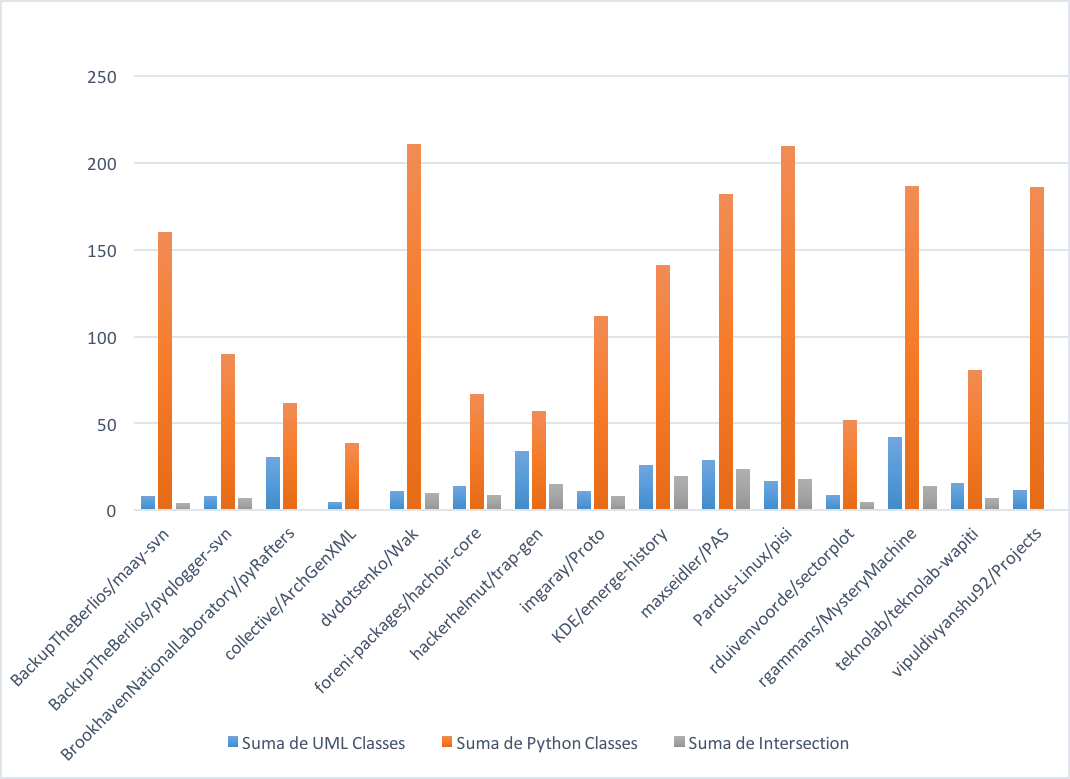
\includegraphics[width=\textwidth, keepaspectratio]{img/GraficasResultados/extracto}
  \caption{Extracto de análisis de proyectos}
  \label{fig:extracto}
\end{figure}

Por cada proyecto\footnote{El nombre de proyecto está identificado
por el autor en GitHub y el nombre que le da al proyecto} de la Figura~\ref{fig:extracto} se observan tres barras:
\begin{itemize}
  \item Una barra azul que representa el número total de clases UML de dicho proyecto
  \item Una barra naranja que representa el número total de clases Python de dicho proyecto
  \item Una barra gris que representa el número total de clases Python modeladas en UML de dicho proyecto
\end{itemize}

El tamaño de las barras indica el número de clases para cada caso.

Para esta gráfica se pueden dar tres situaciones:
\begin{itemize}
  \item Los tamaños de las tres columnas sea el mismo. Este sería el caso ideal, el cual significa que todas
  las clases de Python están modeladas en UML. Este caso solo se ha dado en un proyecto identificado como
  \textit{aydevosotros/TFG-AntonioMolina}.
  \item El tamaño de la columna naranja es mayor que la columna azul. Este es el caso más común, el cual significa
  si la columna gris es del mismo tamaño que la columna azul, que hay clases de Python que no están modeladas en UML.
  Si la columna gris es de menor tamaño que la columna azul, además de lo anterior, significaría que hay algunas clases de UML
  que no están asociadas a alguna clase de Python.
  \item El tamaño de la columna azul es mayor que la columna naranja. Es un caso poco común, el cual se ha dado en
  13 proyectos. Esto significa que tiene más clases de UML que clases en Python. De los 13 proyectos se observa,
  que aún teniendo más clases de UML que de Python, no todas sus clases de Python están modeladas en UML, tal como podemos
  observar en la Figura~\ref{fig:listamasuml}.

  \begin{figure}[htb]
    \centering
    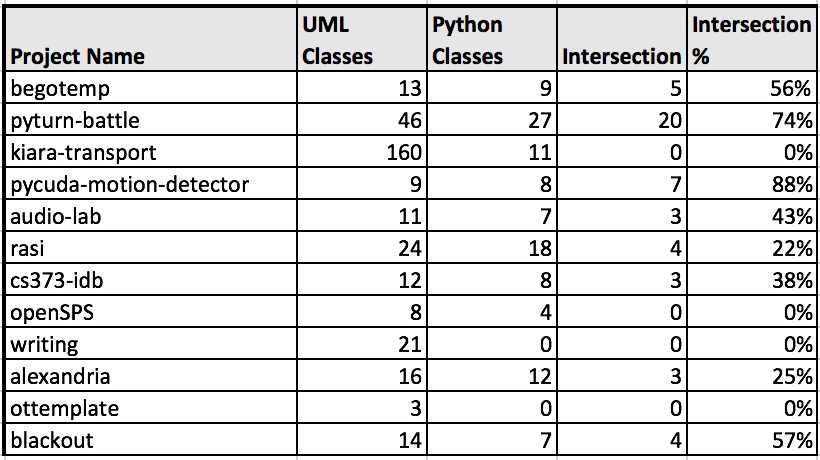
\includegraphics[width=10cm, keepaspectratio]{img/GraficasResultados/listamasuml}
    \caption{Proyectos con más clases UML que Python}
    \label{fig:listamasuml}
  \end{figure}
\end{itemize}

En conclusión, tal como hemos podido suponer en el apartado \ref{subsec:analisistotalproyectos}, gran parte
de las clases de Python no están modeladas en UML.

\section{Porcentaje de intersección frente a número de clases de Python}
\label{subsec:intersecvsclases}

Para poder ver la tendencia general del modelado de UML en base a clases de Python, se representa el porcentaje de
la intersección entre clases UML y Python frente al número total de clases Python.

\begin{figure}[htb]
  \centering
  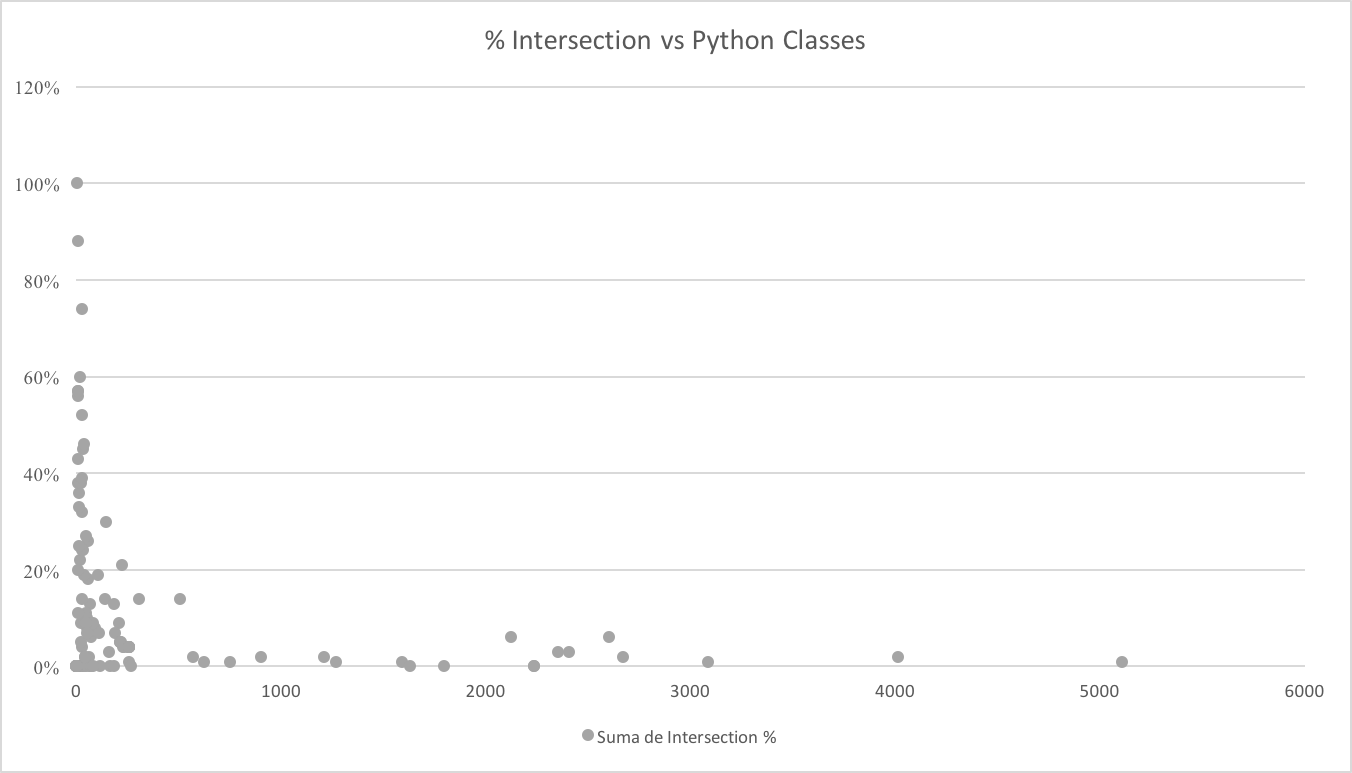
\includegraphics[width=\textwidth, keepaspectratio]{img/GraficasResultados/intersectionvsclass}
  \caption{Intersección vs número clases Python}
  \label{fig:intersectionvsclass}
\end{figure}

Cada punto representa a un proyecto, situado en el porcentaje de la intersección (linea vertical) y en el número total
de clases de Python (linea horizontal) de las que forman el proyecto.

Se puede observar que los mayores porcentajes de intersección se obtienen para aquellos proyectos que tienen pocas
clases a modelar, tal como observamos en el lado izquierdo de la gráfica en el que aparece multitud de puntos, y que ningún proyecto con un número superior a 500 clases presenta un porcentaje mayor al 10\%, tal como observamos en el resto de la gráfica donde aparecen algunos puntos muy dispersos.

En conclusión, se modelan más con UML las clases de Python, cuando hay un número menor de clases de Python a modelar.

\section{Correcciones}
\label{subsec:correcciones}
Las correcciones aplicadas representan un 13,10\% de la intersección de clases UML y Python, tal como hemos visto en la figura
\ref{fig:tablaresultados}. Para dos proyectos de ejemplo se obtiene la Figura~\ref{fig:TFGA-M,pySLD}.

\begin{figure}[htb]
  \centering
  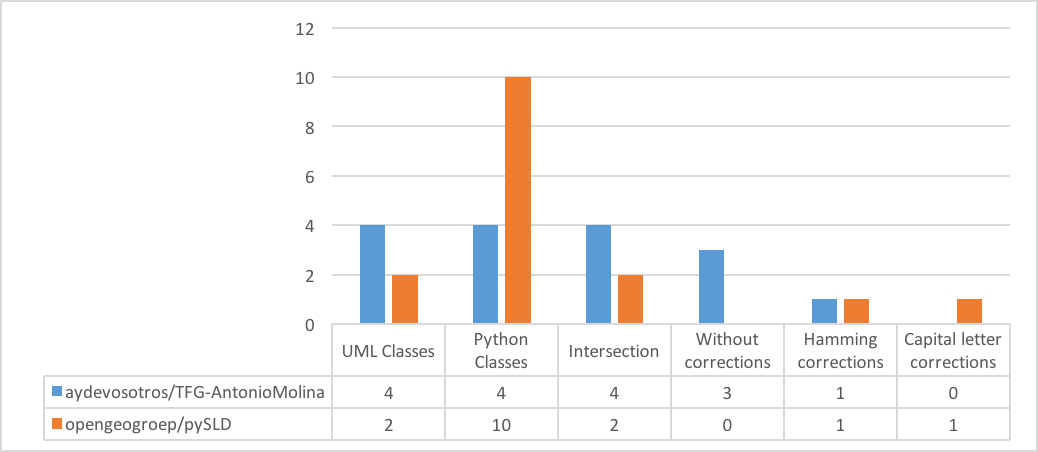
\includegraphics[width=\textwidth, keepaspectratio]{img/GraficasResultados/TFGA-M,pySLD}
  \caption{Proyectos de ejemplo de correcciones}
  \label{fig:TFGA-M,pySLD}
\end{figure}

Para el proyecto identificado como \textit{aydevosotros/TFG-AntonioMolina}, tras las correcciones se obtiene
un 100\% de modelado UML.

Para el proyecto identificado como \textit{opengeogroep/pySLD}, tras las correcciones se modelan dos clases de Python,
que no estaban modeladas antes de la corrección.

%%%%%%%%%%%%%%%%%%%%%%%%%%%%%%%%%%%%%%%%%%%%%%%%%%%%%%%%%%%%%%%%%%%%%%%%%%%%%%%%
%%%%%%%%%%%%%%%%%%%%%%%%%%%%%%%%%%%%%%%%%%%%%%%%%%%%%%%%%%%%%%%%%%%%%%%%%%%%%%%%
% CONCLUSIONES %
%%%%%%%%%%%%%%%%%%%%%%%%%%%%%%%%%%%%%%%%%%%%%%%%%%%%%%%%%%%%%%%%%%%%%%%%%%%%%%%%

\cleardoublepage
\chapter{Conclusiones}
\label{chap:conclusiones}

El desarrollo de este trabajo ha concluido en la creación de una aplicación web para analizar proyectos,
tal como se ha ido explicando a lo largo de la memoria, siendo esta aplicación una aplicación piloto.

Se trata de una primera versión de una herramienta para uso de desarrolladores e investigadores,
la cual se espera que sea de apoyo para ellos, para poder facilitar sus labores en base a los estudios
realizados respecto al uso de UML.

Esta aplicación ya ha servido para analizar el repositorio de proyectos facilitados por el profesor,
y poder hacer una interpretación de los resultados obtenidos. El disponer de estos proyectos verificados
que tenían algo de UML, ha servido para la optimización de la aplicación al ser probada con distintas proyectos,
los cuales presentaban peculiaridades diferentes, con los que se observaban errores que se han ido corrigiendo.

En definitiva, se presenta una aplicación que ya ha sido usada para el desarrollo del trabajo y presentar resultados concretos,
y poder usarse a posteriori para nuevos proyectos que puedan aparecer.

\section{Consecución de objetivos}
\label{sec:consecucion-objetivos}

El objetivo general del trabajo era la realización de una aplicación web, a la cual se le
indicaba una URL de un proyecto de GitHub, y esta devolvía unos parámetros para poder
entender el uso de UML. Este objetivo, tal como se ha ido mostrando a lo largo del proyecto
se ha cumplido totalmente. Además, se ha añadido la funcionalidad de poder consultar todos los
proyectos ya analizados anteriormente.

Respecto a los objetivos específicos, se han cumplido todos, ya que se tratan de objetivos
básicos para la realización de la aplicación web.

\begin{itemize}
  \item Se realizó un estudio de UML, y su presentación en archivos para poder extraer el nombre
  de las clases de esos archivos.
  \item Tras concretar el número de proyectos disponibles sobre los cuáles podríamos trabajar,
  se optimizó el código para proyectos futuros.
  \item Para la presentación de los resultados y poder seguir haciendo uso de la aplicación de manera sencilla,
  se ha creado una aplicación web.
\end{itemize}


\section{Aplicación de lo aprendido}
\label{sec:aplicacion}

A lo largo del grado he tenido distintas asignaturas sobre programación, pero en el desarrollo de esta aplicación,
debido a las tecnologías utilizadas hay que destacar:

\begin{enumerate}
  \item Protocolos para la transmisión de audio y vídeo, en la cual aprendí sobre el uso de Python y el uso de sus bibliotecas.
  \item Laboratorios de tecnologías audiovisuales en la web, en la cual aprendí sobre el desarrollo web tanto del lado cliente
  como del lado servidor, con tecnologías usadas en el proyecto (Django, CSS, JavaScript, HTML5)
\end{enumerate}

También he de destacar mi periodo de prácticas curriculares, en el cuál destacó:
\begin{enumerate}
  \item El aprendizaje que obtuve sobre Microsoft Excel, para el análisis de información a gran escala y la creación de gráficos
  para poder interpretar dicha información.
  \item Capacidad de trabajo autónomo, con resolución de cuestiones con búsquedas en internet o libros.
  \item Planificación de un proyecto.
\end{enumerate}

Y a modo general, debido al carácter de mi grado que se encuentra en constante desarrollo y cambio, me ha servido para estar
preparado a nuevas tecnologías que se puedan presentar sin que ello suponga un gran problema, sino que sea una oportunidad para
estar aprendiendo y no quedarse obsoleto.


\section{Lecciones aprendidas}
\label{sec:lecciones_aprendidas}

Este trabajo me ha servido para adquirir nuevos conocimientos o para profundizar en algunos que se habían utilizado a lo largo del grado.

\begin{enumerate}
  \item Como tema principal del proyecto, UML, he tenido que aprender y entender cual es la motivación de su uso,
  el porque de su importancia y sus ventajas e inconvenientes.
  Aunque el alcance de este proyecto se basa en las clases de UML de los diagramas de clases, este tiene un alcance mucho mayor.
  \item El uso de bases de datos, ya que he tenido que profundizar más en su uso, mediante consultas para la recuperación de información
  de los resultados del proyecto.
  \item Django. Conocía Django de la asignatura de Tecnologías web, pero el proyecto me ha servido para hacer un uso más profundo,
  y creando una web a mi gusto, con un estilo totalmente libre.
  \item La creación de la memoria con \LaTeX{}. El desarrollo de esta memoria se ha realizado con \LaTeX{}, herramienta que nunca había
  utilizado. Aunque al principio cuesta adaptarse, se obtienen resultados muy buenos de aspecto, de manera sencilla una vez conoces su sintaxis.
\end{enumerate}


\section{Trabajos futuros}
\label{sec:trabajos_futuros}

Al tratarse de una herramienta piloto, presenta varios trabajos a futuro, para poder ampliar el uso de esta aplicación.

\begin{enumerate}
  \item \textbf{Ampliar a más lenguajes de programación.} Actualmente solo sirve para analizar proyectos que
  están escritos en Python. Una posible mejora sería ampliar a más lenguajes. El número de lenguajes posibles
  estaría limitado a la herramienta Ctags, que es la encargada de extraer las etiquetas de las clases, y dicha herramienta
  está preparada para un número concreto de lenguajes de programación.
  \item \textbf{Aumentar la complejidad del análisis UML.} En este aspecto existe un mundo de mejora, en el que vamos a plantear posibles
  mejoras que sean de utilidad:
  \begin{itemize}
    \item Valorar no solo por el nombre de la clase, sino por los métodos y atributos que esta tenga.
    \item Establecer posibles relaciones como agregación, herencia, composición...
    \item Actualmente solo nos fijamos en archivos .xmi de UML, que son los estandarizados. Podemos extraer información de otros
    archivos tales como los .uml o de imágenes, ya que es común presentar el modelado de UML en una imagen.
    Esto ampliaría el alcance ya que de la lista de archivos de UML facilitada por el tutor, hay 8106 archivos de UML. De los cuales,
    204 son los que tienen una extensión de .xmi y quedan reducidos a 108 proyectos.
    261 archivos equivalen a la extensión .uml, y el resto, 7641 corresponden a archivos de imagen (.gif, .png, .svg \ldots )
  \end{itemize}
  \item \textbf{Agregar elementos a la web.} Mejoras para la experiencia de usuario como poder descargar un listado de los proyectos
  ya analizados en Excel, calcular el tiempo estimado en base al peso total del proyecto, enviar los resultados por correo para que no se
  tenga que esperar con la página abierta \ldots
\end{enumerate}


\section{Valoración personal}
\label{sec:valoracion}

Desde un primer momento, no sabía sobre que enfocar mi TFG, lo único que tenía claro era que me gustaba programar y
quería hacer algo sobre el desarrollo de un programa, y que no solo estuviese formado por una parte \emph{back-end}, sino por la parte \emph{front-end} también.

Para poder desarrollar algo así, pregunté a los profesores que han dado clase y a los que les gusta la programación, hasta que mi tutor me comentó la posibilidad de realizar
este trabajo. Aunque era un tema que no conocía, me llamó la atención el alcance que podría tener, y que realmente se le podría dar
uso a esta aplicación, por lo que decidí elegir este tema.

He aprendido el proceso completo de documentación y creación de una aplicación web, lo cual me servirá para el mundo laboral.


%%%%%%%%%%%%%%%%%%%%%%%%%%%%%%%%%%%%%%%%%%%%%%%%%%%%%%%%%%%%%%%%%%%%%%%%%%%%%%%%
%%%%%%%%%%%%%%%%%%%%%%%%%%%%%%%%%%%%%%%%%%%%%%%%%%%%%%%%%%%%%%%%%%%%%%%%%%%%%%%%
% APÉNDICE(S) %
%%%%%%%%%%%%%%%%%%%%%%%%%%%%%%%%%%%%%%%%%%%%%%%%%%%%%%%%%%%%%%%%%%%%%%%%%%%%%%%%

\cleardoublepage
\appendix
\chapter{Manual de usuario}
\label{app:manual}

\section{Instalación del servidor}
\label{sec:inst_server}
Para poder iniciar el servidor es necesario tener instalado:

\begin{itemize}
  \item Python
  \item Exuberant Ctags. Para instalarlo hay que ejecutar:
  \begin{lstlisting}
    ~$ sudo apt-get install exuberant-ctags
  \end{lstlisting}
  \item Django. Para instalarlo hay que ejecutar:
  \begin{lstlisting}
    ~$ pip install Django==1.10.6
  \end{lstlisting}
\end{itemize}

Una vez instalado todo lo necesario, desde la carpeta donde se encuentra el proyecto se ejecuta lo siguiente:
\begin{lstlisting}
  ~$ python manage.py runserver
\end{lstlisting}
De esta manera nuestro servidor ya empieza a escuchar en el puerto 8000 (\emph{default}). Para ir a la página principal del proyecto hay que acceder, desde el navegador, a 127.0.0.1:8000.

%%%%%%%%%%%%%%%%%%%%%%%%%%%%%%%%%%%%%%%%%%%%%%%%%%%%%%%%%%%%%%%%%%%%%%%%%%%%%%%%
%%%%%%%%%%%%%%%%%%%%%%%%%%%%%%%%%%%%%%%%%%%%%%%%%%%%%%%%%%%%%%%%%%%%%%%%%%%%%%%%
% BIBLIOGRAFIA %
%%%%%%%%%%%%%%%%%%%%%%%%%%%%%%%%%%%%%%%%%%%%%%%%%%%%%%%%%%%%%%%%%%%%%%%%%%%%%%%%

\cleardoublepage

% Las siguientes dos instrucciones es todo lo que necesitas
% para incluir las citas en la memoria
\bibliographystyle{abbrv}
\bibliography{memoria}

\nocite{*}

% memoria.bib es el nombre del fichero que contiene
% las referencias bibliográficas. Abre ese fichero y mira el formato que tiene,
% que se conoce como BibTeX. Hay muchos sitios que exportan referencias en
% formato BibTeX. Prueba a buscar en http://scholar.google.com por referencias
% y verás que lo puedes hacer de manera sencilla.
% Más información:
% http://texblog.org/2014/04/22/using-google-scholar-to-download-bibtex-citations/

\end{document}
